\documentclass[a4paper, 12pt, oneside]{article}

%% ═════════════════════════════════════════════════════════════════════════
%%  RAPPORT DE MISSION DE FIN D'ÉTUDES — ESTIA, promotion 2026
%%  John HOARAU · ALTEN Sud-Ouest, Direction de l'Innovation, Lab de Toulouse
%%
%%  Structure imposée par « Consignes évaluations Alternance 5 et MFE
%%  2025-2026 », §6.2.3. Rédigé en anglais, à l'exception du paragraphe RSE
%%  (§6.2.3.2 : « Ce paragraphe est à rédiger en français ») et du résumé,
%%  fourni en français, anglais et espagnol comme exigé.
%%
%%  DÉPENDANCES PARTAGÉES, jamais dupliquées :
%%    images       ../BST_DISCO_JH_2026/Images  et  ../Thesis_Cranfield_JH_2026/Images
%%    bibliographie ../BST_DISCO_JH_2026/Utilities/Bibliography.bib
%%                  ../Thesis_Cranfield_JH_2026/Utilities/Bibliography_thesis.bib
%%    glossaire    ../BST_DISCO_JH_2026/Sections/Appendices/Glossary.tex
%% ═════════════════════════════════════════════════════════════════════════

\usepackage[utf8]{inputenc}
\usepackage[T1]{fontenc}
\usepackage[english,french]{babel}
\usepackage{microtype}
\usepackage[sfdefault,lining]{carlito}

%% ── Couleurs de la charte ALTEN (Brandbook 2025) ────────────────────────
\usepackage{xcolor}
\definecolor{altenAzure}{HTML}{008BD2}
\definecolor{altenNavy}{HTML}{043962}
\definecolor{altenAzureDark}{HTML}{176F98}
\definecolor{altenAzureLight}{HTML}{7DCAED}
\definecolor{altenOchreDark}{HTML}{FFBA00}
\definecolor{altenOchrePale}{HTML}{FFEF86}
\definecolor{altenGreyLine}{HTML}{CDCEDA}
\definecolor{altenBlueBg}{HTML}{EBF3F9}
\definecolor{altenBlueBg2}{HTML}{DAE8F3}

\usepackage{sectsty}
\sectionfont{\color{altenNavy}}
\subsectionfont{\color{altenAzureDark}}
\subsubsectionfont{\color{altenAzureDark}}
\paragraphfont{\color{altenNavy}}

%% ── Mise en page ────────────────────────────────────────────────────────
\usepackage[a4paper, top=2.6cm, bottom=2.6cm, left=2.7cm, right=2.7cm,
            footskip=1.1cm]{geometry}
\usepackage[skip=8pt plus 2pt, indent=0pt]{parskip}

\renewcommand{\topfraction}{0.9}
\renewcommand{\bottomfraction}{0.7}
\renewcommand{\textfraction}{0.12}
\renewcommand{\floatpagefraction}{0.75}

%% Rapport confidentiel : marquage sur chaque page, exigé par ALTEN
\pagestyle{plain}
\usepackage{fancyhdr}
\fancypagestyle{plain}{
    \fancyhf{}
    \fancyfoot[R]{\ShortTitle\\\textbf{Document confidentiel}}
    \fancyfoot[L]{ESTIA \textbar{} ALTEN Sud-Ouest\\Mission de fin d'\'etudes 2026}
    \fancyfoot[C]{\thepage}
    \renewcommand{\headrulewidth}{0pt}
    \renewcommand{\footrulewidth}{1pt}
}

%% Sommaire : trois niveaux de titre au maximum (consignes §6.2.3.1)
\setcounter{tocdepth}{3}
\setcounter{secnumdepth}{3}

%% ── Bibliographie partagée ──────────────────────────────────────────────
\usepackage[style=iso-authoryear, backend=biber, sorting=nyt,
            maxbibnames=3, minbibnames=1, giveninits=true,
            urldate=iso]{biblatex}
\addbibresource{../BST_DISCO_JH_2026/Utilities/Bibliography.bib}
\addbibresource{../Thesis_Cranfield_JH_2026/Utilities/Bibliography_thesis.bib}
\addbibresource{Utilities/Bibliography_mfe.bib}
\usepackage[nottoc,numbib]{tocbibind}

%% ── Glossaire partagé ───────────────────────────────────────────────────
\usepackage[acronym, section=subsection]{glossaries}
\makenoidxglossaries{}
%% ─────────────────────────────────────────────────────────────────────────
%%  ACRONYMS
%% ─────────────────────────────────────────────────────────────────────────
\newacronym{ahp}{AHP}{Analytic Hierarchy Process}
\newacronym{bst}{BST}{Bilan Scientifique et Technique}
\newacronym{bwm}{BWM}{Best-Worst Method}
\newacronym{ci}{CI}{Consistency Index}
\newacronym{cr}{CR}{Consistency Ratio}
\newacronym{csrd}{CSRD}{Corporate Sustainability Reporting Directive}
\newacronym{dag}{DAG}{Directed Acyclic Graph}
\newacronym{din}{DIN}{Direction Innovation Num\'erique}
\newacronym{disco}{DISCO}{Supply Chain Illustrator (Digital Twin, DIN ALTEN)}
\newacronym{dt}{DT}{Digital Twin}
\newacronym{fbwm}{F-BWM}{Fuzzy Best-Worst Method}
\newacronym{glec}{GLEC}{Global Logistics Emissions Council}
\newacronym{hgv}{HGV}{Heavy Goods Vehicle}
\newacronym{iot}{IoT}{Internet of Things}
\newacronym{ipg}{IPG}{Itinerary Performance Index}
\newacronym{kpi}{KPI}{Key Performance Indicator}
\newacronym{lppl}{LPPL}{Log-Periodic Power Law}
\newacronym{mcdm}{MCDM}{Multi-Criteria Decision-Making}
\newacronym{mts}{MTS}{Manchester Triage System}
\newacronym{pi}{PI}{Physical Internet}
\newacronym{promethee}{PROMETHEE}{Preference Ranking Organisation METHod for Enrichment Evaluation}
\newacronym{ri}{RI}{Random Index (Saaty)}
\newacronym{sc}{SC}{Supply Chain}
\newacronym{tmt}{TMT}{Temporal Motivational Theory}
\newacronym{tfn}{TFN}{Triangular Fuzzy Number}
\newacronym{tts}{TTS}{Time To Service}
\newacronym{ttr}{TTR}{Time To Recovery}
\newacronym{vecto}{VECTO}{Vehicle Energy Consumption calculation TOol}
\newacronym{xai}{XAI}{Explainable Artificial Intelligence}

%% ─────────────────────────────────────────────────────────────────────────
%%  MAIN GLOSSARY ENTRIES (key mathematical symbols and concepts)
%% ─────────────────────────────────────────────────────────────────────────
\newglossaryentry{ur}{
    name={$U_r(t)$},
    description={Real (operationally computable) urgency at time $t$: a
        weighted probabilistic OR aggregation of six local KPI blocks
        (time, capacity, performance, risk, cost, CO2), $U_{r,\text{local}}
        = 1-\prod_m(1-u_m)^{\omega_m}$, propagated upstream across the
        supply chain DAG through the leaky coefficients $\beta_{ji}$}}

\newglossaryentry{ud}{
    name={$U_d$},
    description={Declared urgency, a scalar $\in [0,1]$ elicited from the
        human operator via an AHP or Fuzzy-BWM questionnaire, propagated
        downstream across the supply chain DAG through the leaky
        coefficients $\gamma_{ik}$}}

\newglossaryentry{at}{
    name={$A(t)$},
    description={Adequacy score at time $t$, quantifying the asymmetric
        Prospect Theory penalty between $U_d$ and $U_r(t)$:
        $A = 100\times(\exp(-\text{penalty})-\text{floor})/(1-\text{floor})$
        with $\text{penalty}=\lambda_{\text{under}}H^{\alpha}+
        \lambda_{\text{over}}F^{\alpha}$, $\in [0,100]$}}

\newglossaryentry{deltau}{
    name={$\Delta U(t)$},
    description={Raw urgency mismatch: $U_d - U_r(t) \in (-1,1)$; positive
        = over-triage (false urgency), negative = under-triage
        (hidden risk)}}

\newglossaryentry{fh}{
    name={$F$, $H$},
    description={False urgency $F=[U_d-U_r]_+$ (unjustified panic) and
        hidden risk $H=[U_r-U_d]_+$ (silent danger), the two asymmetrically
        penalised pathologies underlying $A(t)$}}

\newglossaryentry{omegam}{
    name={$\omega_m$},
    description={Aggregation weight of KPI block $m$ in the real urgency
        noisy-OR aggregation, reused unchanged as the PROMETHEE~II
        criteria weight for network-wide node outranking}}

\newglossaryentry{deltaurcrit}{
    name={$\Delta U_{r,\text{final}}$},
    description={Network criticality delta: the increase in real urgency
        propagated to final-customer nodes when a given node's local
        urgency is forced to saturation in a systematic shock simulation}}


\usepackage{amsmath, amssymb, mathtools}

%% ── Figures : les deux arbres d'images sont partagés, jamais copiés ─────
\usepackage{graphicx}
\graphicspath{{./}{../BST_DISCO_JH_2026/}{../Thesis_Cranfield_JH_2026/}}
\usepackage{caption}
\captionsetup{labelfont={bf,color=altenNavy}, textfont={color=altenNavy},
              font=small}
\usepackage[hidelinks]{hyperref}
\hypersetup{colorlinks=true, linkcolor=altenAzure, citecolor=altenAzure,
            urlcolor=altenAzure,
            pdftitle={Mesurer l'ecart entre urgence declaree et urgence reelle},
            pdfauthor={John Hoarau}}

\usepackage{tabularx, array, booktabs, multirow, longtable, float}
\usepackage{colortbl}
\arrayrulecolor{altenNavy}
\renewcommand{\tabularxcolumn}[1]{m{#1}}

\usepackage{enumitem}
\setitemize{parsep=0pt, partopsep=0pt}
\setenumerate{parsep=0pt, partopsep=0pt}

%% ── Encadrés de la charte ───────────────────────────────────────────────
\usepackage[strict]{changepage}
\usepackage{framed}

\colorlet{definitionshade}{altenBlueBg2}
\newenvironment{definitionBox}{%
  \def\FrameCommand{\hspace{1pt}{\color{altenNavy}\vrule width 2pt}%
    {\color{definitionshade}\vrule width 4pt}\colorbox{definitionshade}}%
  \MakeFramed{\advance\hsize-\width\FrameRestore}%
  \noindent\hspace{-4.55pt}\begin{adjustwidth}{}{7pt}\vspace{4pt}%
}{\vspace{2pt}\end{adjustwidth}\endMakeFramed}

\colorlet{attentionShade}{altenOchrePale!45!white}
\newenvironment{attentionBox}{%
  \def\FrameCommand{\hspace{1pt}{\color{altenOchreDark}\vrule width 2pt}%
    {\color{attentionShade}\vrule width 4pt}\colorbox{attentionShade}}%
  \MakeFramed{\advance\hsize-\width\FrameRestore}%
  \noindent\hspace{-4.55pt}\begin{adjustwidth}{}{7pt}\vspace{4pt}%
}{\vspace{2pt}\end{adjustwidth}\endMakeFramed}

%% Le paragraphe RSE est exige en francais ; sa traduction anglaise le suit
%% immediatement pour que le document reste lisible de bout en bout.
\colorlet{frShade}{altenBlueBg}
\newenvironment{frenchBox}{%
  \def\FrameCommand{\hspace{1pt}{\color{altenAzure}\vrule width 2pt}%
    {\color{frShade}\vrule width 4pt}\colorbox{frShade}}%
  \MakeFramed{\advance\hsize-\width\FrameRestore}%
  \noindent\hspace{-4.55pt}\begin{adjustwidth}{}{7pt}\vspace{4pt}%
  \selectlanguage{french}%
}{\vspace{2pt}\end{adjustwidth}\endMakeFramed\selectlanguage{english}}

\begin{document}
\selectlanguage{english}
\color{altenNavy}

\newcommand{\ShortTitle}{MFE 2026 · Declared vs.\ Real Urgency}

%% Page de garde reprenant tous les elements du modele ESTIA
%% (« Rapport - modele de document - v2025-2026.docx ») : logo entreprise,
%% titre, entreprise, NOM Prenom + promotion, periode, numero de stage,
%% mention de confidentialite, tuteurs entreprise et ESTIA, thematique.
\begin{titlepage}
    \centering

    
\includegraphics[height=1.7cm, keepaspectratio]{Images/0.Cover/LogoALTEN.png}
    \hspace{1cm}
    
\includegraphics[height=1.7cm, keepaspectratio]{Images/0.Cover/LogoDIN.png}
    \hspace{1cm}
    
\includegraphics[height=1.7cm, keepaspectratio]{Images/0.Cover/LogoESTIA.png}
    \vspace{0.5cm}

    {\Large\bfseries
        Measuring the Gap Between Declared\\[4pt]
        and Real Urgency in a Supply Chain\\[4pt]
        Digital Twin\par}

    \vspace{0.5cm}
    {\normalsize\itshape A decision-support layer for the Smart Green Supply
        Chain programme\par}

    \vspace{0.5cm}
    {\large ALTEN Sud-Ouest \textbar{} Direction de l'Innovation\par}
    {\normalsize Lab de Toulouse\par}

    \vspace{0.5cm}
    {\large\bfseries HOARAU John\par}
    {\normalsize Promotion 2026 \textbar{} Cycle Ing\'enieur 3\textsuperscript{e} ann\'ee\par}
    {\normalsize Parcours double dipl\^ome Cranfield University (DED)\par}

    \vspace{0.5cm}
    {\normalsize P\'eriode du 13 avril 2026 au 16 octobre 2026\par}
    {\normalsize 3\textsuperscript{e} ann\'ee \textbar{} Mission de fin d'\'etudes\par}

    \vspace{0.5cm}
    {\normalsize\bfseries Rapport confidentiel : OUI\par}

    \vfill

    {\normalsize
        \renewcommand{\arraystretch}{1.25}
        \begin{tabularx}{\textwidth}{@{}>{\raggedright\arraybackslash}p{5.9cm} X@{}}
        \toprule
        \multicolumn{2}{@{}l}{\textbf{Encadrement}} \\
        \midrule
        Tuteur entreprise & \textbf{S\'ebastien PERTHUISOT} \newline
            Directeur de Programme de Recherche, \newline
            Expert Qualit\'e \& Supply Chain, DIN \\
        Tuteur entreprise & \textbf{Fabien JULES} \newline
            Charg\'e Innovation, ALTEN \\
        Tuteur ESTIA & \textbf{Dr. David GOMEZ} \newline
            Enseignant-chercheur en informatique \\
        Tuteur CRANFIELD & \textbf{Dr. Peter Sherar} \newline
            Enseignant-chercheur en informatique \\
        \midrule
        \multicolumn{2}{@{}l}{\textbf{Th\'ematique du travail r\'ealis\'e}} \\
        \midrule
        \multicolumn{2}{@{}l}{Informatique \textbar{} G\'enie industriel} \\
        \bottomrule
    {\footnotesize ESTIA -- \'Ecole Sup\'erieure des Technologies Industrielles
        Avanc\'ees, Technopole Izarbel, 64210 Bidart\par}

        \end{tabularx}\par}


\end{titlepage}


\clearpage
\pagenumbering{roman}
\section*{Acknowledgements}
\label{sec:remerciements}
\addcontentsline{toc}{section}{Acknowledgements}

My thanks go first to \textbf{S\'ebastien Perthuisot}, Research Programme Director,
Quality \& Supply Chain Expert at the Direction de l'Innovation, who set the direction of
this work and then left me room to take it somewhere. The weekly
review he held with me was where most of the difficult questions in this report were first
asked.

I thank \textbf{\'Emilienne Lardy} and  \textbf{Selma Ferhat} , who ran the scrum and planning cadence that gave the
six months their rhythm, and whose reviews repeatedly sent me back to check a claim I had
been ready to make. I thank them also for their scientific supervision.

I thank \textbf{Liam Jones}, who worked on the network representation side of the same
programme. Sharing a weekly demo with someone solving a neighbouring problem did more for
the quality of my own work than any amount of solitary effort would have.

I thank \textbf{Dr David Gomez} of ESTIA for the academic supervision and framing of this
mission, and \textbf{Dr Peter Sherar} of Cranfield University for supervising the research
strand that ran alongside it.

Finally, I thank the whole Direction de l'Innovation team at the Toulouse Lab for the
welcome, and my family for their support across the whole of this engineering degree.


\clearpage
\section*{R\'esum\'e}
\label{sec:resume_fr}
\addcontentsline{toc}{section}{R\'esum\'e / Abstract / Resumen}

\begin{otherlanguage}{french}
Dans une cha\^ine d'approvisionnement, l'urgence qu'un op\'erateur d\'eclare diverge souvent
de celle que l'on calcule depuis l'\'etat op\'erationnel r\'eel. Sur-d\'eclarer gaspille une
capacit\'e partag\'ee~; sous-d\'eclarer laisse un risque de rupture invisible. Aucun jumeau
num\'erique, publi\'e ou brevet\'e, ne mesure encore cet \'ecart.

Cette mission, men\'ee \`a la Direction de l'Innovation d'ALTEN, a con\c{c}u et \'eprouv\'e
une couche logicielle qui le mesure, livr\'ee sous le nom de \textbf{SupplyScore}.
L'urgence r\'eelle est agr\'eg\'ee depuis six blocs
d'indicateurs par une r\`egle \emph{non compensatoire}~: le bloc le plus d\'egrad\'e tire le
score vers son maximum, sans qu'un bloc sain puisse l'en emp\^echer. Elle est ensuite
propag\'ee sur le r\'eseau. L'urgence d\'eclar\'ee, elle, est \'elicit\'ee par un
questionnaire de comparaisons par paires contr\^ol\'e en coh\'erence, et l'\'ecart entre les
deux est not\'e sur $[0,100]$.

Dans les tests de \emph{serious game} r\'ealis\'es, sur les six tours pr\'ec\'edant la mise au
jour d'une crise, l'\'ecart d\'esigne trois n\oe{}uds, tous trois futurs d\'efaillants, sans
une seule fausse alerte~; le plus mal not\'e est signal\'e huit tours avant de rater son
jalon, alors que son responsable d\'eclare une urgence de $0{,}001$.

Trois \'epreuves ind\'ependantes en ont d\'elimit\'e la port\'ee~: elles ont localis\'e un
d\'efaut pr\'ecis de la couche de pr\'evision, \'etabli que l'outil rep\`ere celui qui se
m\'eprend sur son \'etat et non celui qui le tait, et mesur\'e o\`u la simulation apporte
r\'eellement sa valeur.

\medskip

\noindent\textbf{Mots-cl\'es~:} jumeau num\'erique de cha\^ine d'approvisionnement,
ad\'equation d'urgence, biais cognitif, aide multicrit\`ere \`a la d\'ecision, calibration de
pr\'evisions, biais d'automatisation, \emph{serious game}.
\end{otherlanguage}

\vspace{0.3cm}

\section*{Abstract}
\label{sec:resume_en}

In a supply chain, the urgency an operator declares often diverges from the urgency computable
from the real operational state. Over-declaring wastes shared capacity; under-declaring leaves
rupture risk invisible. No digital twin, published or patented, measures that gap yet.

This mission, carried out at the Direction de l'Innovation of ALTEN, designed and tested a
software layer that measures it, delivered as \textbf{SupplyScore}. Real urgency is
aggregated from six indicator blocks by a
\emph{non-compensatory} rule: the most degraded block drives the score toward its maximum, and
no healthy block can offset it. It is then propagated across the network. Declared urgency is
elicited separately, through a consistency-gated pairwise questionnaire, and the gap between
the two is scored on $[0,100]$.

In the serious-game tests carried out, over the six turns before a crisis becomes public, the
gap flags three nodes, all three of which later miss a delivery commitment, with no false alarm
on any turn; the worst-scoring of them is flagged eight turns before it misses, while its
manager declares an urgency of $0.001$.

Three independent tests then established its domain: they located a precise defect in the
forecast layer, established that the tool detects a declarant who misjudges their own
state rather than one who knows it and stays silent, and measured where the simulation
genuinely adds value.

\medskip

\noindent\textbf{Keywords:} supply chain digital twin, urgency adequacy, cognitive bias,
multi-criteria decision analysis, forecast calibration, automation bias, serious game.

\vspace{0.3cm}

\section*{Resumen}
\label{sec:resume_es}

\begin{otherlanguage}{spanish}
En una cadena de suministro, la urgencia que declara un operador difiere a menudo de la
urgencia calculable a partir del estado operativo real. Declarar de m\'as desperdicia
capacidad compartida; declarar de menos deja invisible el riesgo de ruptura. Ning\'un gemelo
digital, publicado o patentado, mide todav\'ia esa diferencia.

Esta misi\'on, realizada en la Direcci\'on de Innovaci\'on de ALTEN, dise\~n\'o y prob\'o una
capa de software que la mide, entregada con el nombre de \textbf{SupplyScore}. La urgencia
real se agrega a partir de seis bloques de
indicadores mediante una regla \emph{no compensatoria}: el bloque m\'as degradado lleva la
puntuaci\'on hacia su m\'aximo y ning\'un bloque sano puede compensarlo. Despu\'es se propaga
por la red. La urgencia declarada se obtiene por separado, mediante un cuestionario de
comparaciones por pares con control de coherencia, y la diferencia entre ambas se punt\'ua en
$[0,100]$.

En las pruebas de \emph{serious game} realizadas, en los seis turnos previos a que una crisis
se haga p\'ublica, la diferencia se\~nala tres nodos, los tres futuros incumplidores, sin una
sola falsa alarma; el peor puntuado se se\~nala ocho turnos antes de incumplir su hito,
mientras su responsable declara una urgencia de $0{,}001$.

Tres pruebas independientes delimitaron su alcance: localizaron un defecto preciso en la capa
de predicci\'on, establecieron que la herramienta detecta a quien se equivoca sobre su propio
estado y no a quien lo conoce y calla, y midieron d\'onde aporta valor realmente la
simulaci\'on.

\medskip

\noindent\textbf{Palabras clave:} gemelo digital de cadena de suministro, adecuaci\'on de
urgencia, sesgo cognitivo, an\'alisis multicriterio de decisi\'on, calibraci\'on de
predicciones, sesgo de automatizaci\'on, \emph{serious game}.
\end{otherlanguage}


\clearpage
\section*{Preamble}
\label{sec:preambule}
\addcontentsline{toc}{section}{Preamble}

Three points about this document are worth stating before it begins.

\paragraph{Confidentiality.}
The project is designated confidential by ALTEN in the annex to the placement agreement.
This report therefore carries a confidentiality marking on every page. It contains internal
scoring parameters, the architecture of an unreleased software product and results not
published elsewhere. It is submitted to ESTIA for examination only and should not be
circulated further.

\paragraph{Language.}
The report is written in English, which the ESTIA guidelines permit and which matches the
Cranfield double-degree track and the oral defence. Two exceptions follow the guidelines
rather than my preference: the abstract is provided in French, English and Spanish, and the
paragraph on ALTEN's corporate social responsibility policy is written in French as
required. An English translation is placed immediately beside it so that no part of the
document is unreadable to an English-speaking reader.

\paragraph{Relationship to the other documents produced during the mission.}
Three written deliverables came out of this placement, and they are not versions of one
another. A \emph{Bilan Scientifique et Technique} was produced for ALTEN in the company's
own R\&D reporting format. A research thesis was produced for Cranfield University under
its own supervision and rules. The present report is the ESTIA mission report: it covers
the mission as an engineering assignment inside a company, which the other two do not, and
it is organised around the company, the problem, the mission, its organisation and its
outcome. Technical material and figures are shared between the three where the same work is
being described, which the ESTIA guidelines expressly allow, but the structure and the
argument here are specific to this document.


\clearpage
\tableofcontents

\clearpage
\listoffigures

\clearpage
\listoftables

\clearpage
\pagenumbering{arabic}
\section{Introduction}
\label{sec:intro}
A supply chain coordinator opens the week with a list of nodes and a finite amount of
attention. Somewhere on that list is the supplier that will cause next month's line
stoppage. Nothing on the screen says which one it is.

That is the practical shape of the problem this mission addressed. Modern supply chains are
monitored through indicators that each measure one dimension at a time, while the decision
the coordinator actually faces is multi-dimensional: cost against deadline against supplier
reliability against, increasingly, carbon. When the tooling cannot combine those dimensions,
the coordinator combines them by judgment. Judgment is then the real decision layer of the
system, and it is the layer nobody measures.

The consequences are not evenly distributed. Declaring more urgency than a situation
warrants consumes shared transport and production capacity that another flow needed.
Declaring less leaves a risk that nobody is watching, and by the time it becomes visible the
window to act on it has closed. The second error is the more expensive, and it is the harder
one to detect, precisely because an under-declared risk generates no signal.

This mission was carried out at the Direction de l'Innovation of ALTEN, within the Smart
Green Supply Chain research programme, between 13 April and 16 October 2026. Its subject was
the layer that sits before any planning decision: the urgency signal itself. The question
driving the work was whether the gap between what an operator declares and what the
operational state actually supports can be measured well enough, inside a working digital
twin, to be acted upon.

The answer this report reaches is a qualified no, and the value of the work lies in how
precisely that no can be stated. A complete system was delivered and is operational. The
signal it produces was then tested against recorded outcomes rather than asserted, and the
test failed in a way that identifies exactly which component is responsible and what would
repair it. A second measurement, unplanned at the outset, showed that displaying the
system's own forecast to the person making the declaration changed that declaration, and
changed it in the wrong direction at the worst possible moment. Both findings are more
useful to ALTEN than a favourable score would have been.

The report is organised as the mission itself was. Section~\ref{sec:entreprise} presents
ALTEN, the Direction de l'Innovation and the research programme this work sits inside,
including the company's corporate social responsibility policy and how the mission relates
to it. Section~\ref{sec:problematique} states the problem that justified opening the
subject. Section~\ref{sec:mission} gives the assignment, its objectives, its indicators and
its deliverables. Section~\ref{sec:organisation} describes how the project was run: who was
involved, what resources were available, which working method was applied, how the six
months were phased, and which risks were carried. Section~\ref{sec:etatdelart} reviews the
existing methods and identifies what none of them provides.
Section~\ref{sec:realisation} reports the work carried out and what it produced, including
the problems met along the way and how they were resolved. Section~\ref{sec:conclusion}
assesses the results against the objectives, sets out what remains to be done, and closes
with a personal assessment against the ESTIA engineering competency framework.


\clearpage
\section{The Company}
\label{sec:entreprise}
\subsection{The ALTEN Group}
\label{sec:alten}

ALTEN is a French engineering and technology consulting group founded in 1988, with its
head office in Boulogne-Billancourt. It sells engineering expertise rather than products:
its consultants are placed on the technical projects of client companies, across the
aerospace, defence, energy, transport, telecommunications, health and finance sectors. The
group operates in more than thirty countries, and France remains its largest market.

Two features of that model matter for understanding this mission. First, ALTEN's asset is the
technical capability of its people, so anything that raises the level of a whole practice has
leverage that a single client project does not. Second, a consulting group works for many
clients at once, so it sees the same difficulty appear in company after company. That is how
a problem gets recognised as belonging to the industry rather than to one customer, and the
urgency assessment problem treated in this report is one of those.

Figure~\ref{fig:situation} places the mission inside the group, from the whole down to the
one layer this report is about. The rest of this section walks the same path.

\begin{figure}[H]
\centering
\begin{tikzpicture}[
    n/.style  = {bloc, minimum height=0.6cm, font=\scriptsize, align=left,
                 inner xsep=6pt},
    nF/.style = {blocFort, minimum height=0.6cm, font=\scriptsize, align=left,
                 inner xsep=6pt}]

\node[n, text width=11.2cm]  (g1)
  {\textbf{ALTEN Group:} engineering and technology consulting, 1988, thirty countries};
\node[n, text width=10.4cm, below right=1.8mm and 8mm of g1.south west,
      anchor=north west] (g2)
  {\textbf{Direction de l'Innovation:} the group's own R\&D, distinct from client work};
\node[n, text width=9.6cm, below right=1.8mm and 8mm of g2.south west,
      anchor=north west] (g3)
  {\textbf{Toulouse Lab:} one of the ALTEN Labs, where this mission took place};
\node[n, text width=8.8cm, below right=1.8mm and 8mm of g3.south west,
      anchor=north west] (g4)
  {\textbf{Smart Green Supply Chain:} lean, green and predictive aims at once};
\node[n, text width=8.0cm, below right=1.8mm and 8mm of g4.south west,
      anchor=north west] (g5)
  {\textbf{DISCO and its modules:} routing, supplier risk, carbon, transport};
\node[nF, text width=7.2cm, below right=1.8mm and 8mm of g5.south west,
      anchor=north west] (g6)
  {\textbf{This mission:} the urgency layer none of them provides};

\foreach \a/\b in {g1/g2, g2/g3, g3/g4, g4/g5, g5/g6}
  \draw[flecheFine] ($(\a.south west)+(4mm,0)$) |- (\b.west);

\end{tikzpicture}
\caption[Where the mission sits inside ALTEN]{From the group down to the layer this report is
about.}
\label{fig:situation}
\end{figure}

\subsection{The Direction de l'Innovation}
\label{sec:din}

The Direction de l'Innovation (DIN) is the entity responsible for ALTEN's own research and
development, as distinct from the work its consultants deliver to clients. It operates a
network of ALTEN Labs and brings together permanent researchers, doctoral candidates,
consultants, interns and apprentices. Its output is not billable hours but reusable assets:
methods, prototypes and expertise that consultants and clients can subsequently draw on.

This mission took place at the Toulouse Lab, within the Smart Green Supply Chain research
programme, which pursues three aims at once. The lean aim targets waste, meaning cost, delay
and excess stock. The green aim targets the carbon footprint of each transport leg, working to
the Global Logistics Emissions Council (GLEC) Framework
v3.2~\autocite{smartfreight2023glec} and ISO~14083:2023~\autocite{iso14083}. The predictive
aim, where this work sits, targets the anticipation of disruption.

The programme's central artefact is DISCO, a serious game and digital twin simulating a
complete supply chain for a satellite product across 22 component
suppliers~\autocite{baxas2025architecture}. Figure~\ref{fig:disco_map} shows the network
players work with and the three dimensions their decisions are scored on.

\begin{figure}[H]
    \centering
    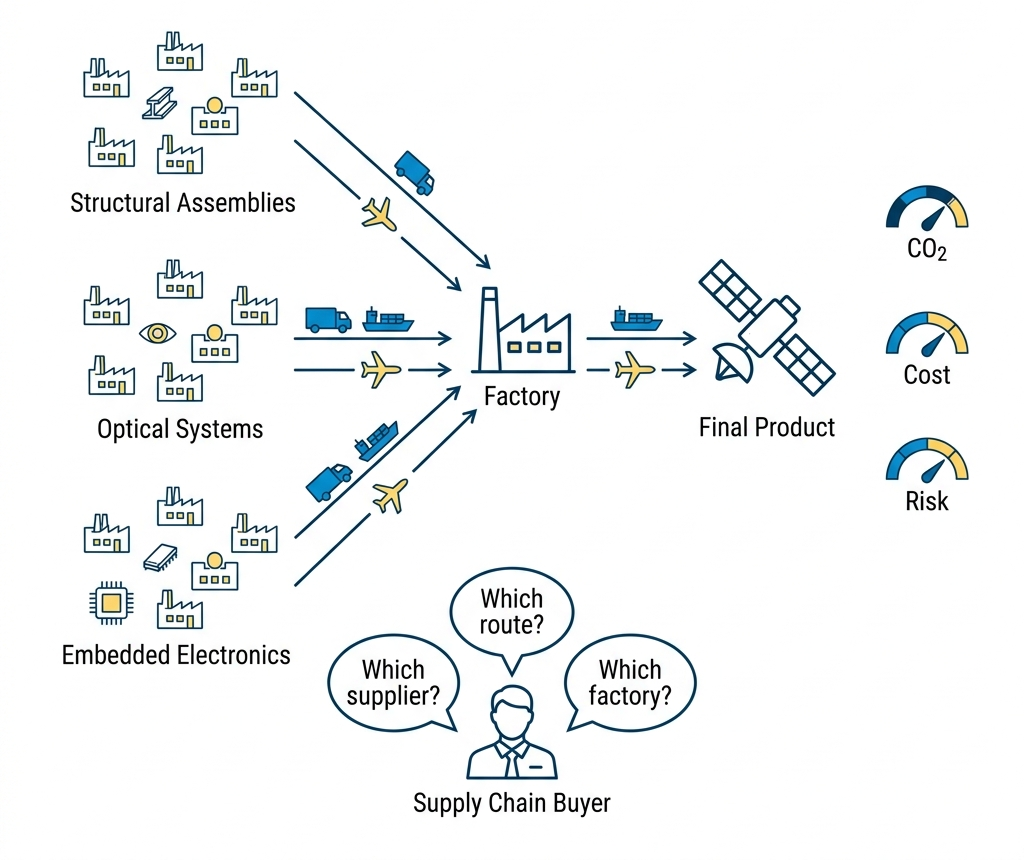
\includegraphics[width=0.52\linewidth]{Images/1.Introduction/disco_map.png}
    \caption[The DISCO serious game network]{The DISCO serious game network. Players hold one
    node each and are scored on cost, delay and carbon.}
    \label{fig:disco_map}
\end{figure}

Successive internships have built its components: the Physical Internet routing
module~\autocite{baulain2024internet}, the supplier risk scorer~\autocite{kabouche2025scoring},
the per-route carbon quantification~\autocite{cordova2024green} and the transport management
interface~\autocite{mondelice2025tms}. The work described here adds a layer none of them
covers, and it ran alongside a parallel internship on the network representation and
geographic modelling side of the same programme, discussed in
Section~\ref{sec:parties_prenantes}. DISCO is the environment the present work was designed to
be compatible with, although the delivered system runs alongside it rather than inside it, for
reasons given in Section~\ref{sec:mission_perimetre}.

\subsection{Politique RSE d'ALTEN \textnormal{\textmd{(CSR policy, in French)}}}
\label{sec:rse}

\begin{frenchBox}
ALTEN a adh\'er\'e au Pacte Mondial des Nations Unies en 2010 et structure depuis sa politique
de responsabilit\'e soci\'etale autour de trois piliers~: l'humain, l'environnement et
l'innovation durable. La d\'emarche se mesure autant qu'elle se d\'eclare~: score EcoVadis de
85/100 en 2025, niveau Platinum et premier centile mondial, note A\textminus{} confirm\'ee au
Carbon Disclosure Project, et trajectoire de r\'eduction valid\'ee par la Science Based Targets
initiative en 2023 avec une neutralit\'e carbone vis\'ee \`a l'horizon 2050.

Sur le pilier humain, le Groupe r\'eunit plus de cent nationalit\'es, a sign\'e les
\emph{Women's Empowerment Principles} des Nations Unies et publie au titre de 2025 un index
d'\'egalit\'e professionnelle de 88/100 pour ALTEN Sud-Ouest, l'entit\'e juridique dans
laquelle s'est d\'eroul\'ee cette mission~; le programme INSPIRE 2026-2030 en porte la suite.
Sur le pilier environnemental, les actions internes sont concr\`etes et v\'erifiables~:
100~\% d'\'electricit\'e renouvelable pour les b\^atiments fran\c{c}ais dont la puissance
souscrite d\'epasse 36~kVA, 80~\% des surfaces couvertes par le tri s\'electif, une
certification ISO~14001 en cours d'extension, et des ateliers Fresque du Climat.

C'est le troisi\`eme pilier qui \'eclaire le mieux cette mission. ALTEN consacre 31~\% de sa
R\&D \`a l'innovation environnementale, et le programme dans lequel ce stage s'est inscrit en
fait partie~: un programme \emph{Smart Green} Supply Chain, o\`u les \'emissions de
CO\textsubscript{2} constituent l'un des six blocs du mod\`ele d'urgence d\'evelopp\'e ici, au
m\^eme rang que le co\^ut ou le d\'elai, et non une correction appliqu\'ee apr\`es coup. La
politique RSE du Groupe n'a donc pas seulement encadr\'e ce travail~: elle en a d\'etermin\'e
une variable de mod\'elisation.

\medskip

\noindent\textbf{Prise de recul.} Le carbone est l'un des six blocs du mod\`ele, et c'est
pourtant celui qui a le moins servi pendant la premi\`ere campagne. La raison n'est pas un
choix de mod\'elisation, c'est un manque de donn\'ees. Les \'emissions par trajet sont
connues \`a l'\'echelle du programme, pas encore \`a celle d'un n\oe{}ud et d'une semaine,
qui est la maille o\`u l'urgence se calcule. Une ambition environnementale peut donc \^etre
inscrite dans un mod\`ele et y rester la dimension la moins active. Avoir montr\'e \`a quel
endroit pr\'ecis la donn\'ee manque est, \`a mon sens, la contribution RSE la plus utile de
cette mission.
\end{frenchBox}


\clearpage
\section{Problem Statement}
\label{sec:problematique}
%% Pourquoi la mission existe : le probleme que l'entreprise a voulu
%% traiter, ferme par une question a laquelle le rapport repond.

\subsection{Why ALTEN Opened This Subject}
\label{sec:pourquoi}

Every component the programme had built by the start of this internship answers a question of
the form \emph{what is the state of this part of the chain?} None answers the question that
comes next. Once the state is known, a coordinator still has to decide where to spend a finite
amount of attention this week, and that decision runs on a signal none of those modules
produces: how urgent each node is. In practice it comes from people. A buyer says a supplier is
critical; a plant says a line is at risk. The twin records the consequence of those judgments
without ever evaluating the judgments themselves.

That is a gap with a cost attached, because the signal is not neutral. Zhu, Yang and Hsee
demonstrate across five controlled experiments that people systematically favour imminent
low-value tasks over distant high-value ones, and that the bias persists even when they are
told about it~\autocite{zhu2018mere}; field studies find the same pattern under
workload~\autocite{rusou2020psychology,diwa2020task}. A twin that consumes a human urgency
declaration as ground truth inherits that bias and propagates it across the network.

\subsection{The Cost of the Two Errors}

The two directions of error are not symmetric, which is what makes the problem worth
instrumenting rather than tolerating. Figure~\ref{fig:asymetrie} sets them side by side.

\begin{figure}[H]
\centering
\begin{tikzpicture}[
    err/.style = {bloc, text width=5.4cm, minimum height=0.82cm, font=\scriptsize},
    errH/.style = {err, fill=altenOchrePale!55!white, draw=altenOchreDark, line width=1pt},
    node distance = 3mm]

\node[blocFort, text width=5.2cm, font=\small] (dec)
     {\textbf{the urgency an operator declares}};

\node[err, below left=11mm and 3mm of dec.south, anchor=north east, fill=altenBlueBg2]
     (f1) {\textbf{too high: false urgency}\\[1pt] $U_d > U_r$};
\node[errH, below right=11mm and 3mm of dec.south, anchor=north west]
     (h1) {\textbf{too low: hidden risk}\\[1pt] $U_d < U_r$};

\node[err, below=of f1] (f2) {consumes expedited transport, premium capacity and the
                              coordinator's attention};
\node[err, below=of h1] (h2) {raises no alert, enters no priority list, consumes no
                              attention};

\node[err, below=of f2] (f3) {the bill lands on another flow, often on another actor
                              entirely};
\node[err, below=of h2] (h3) {surfaces only as a missed delivery, once the window to act on
                              it has closed};

\node[blocPale, text width=5.4cm, minimum height=0.82cm, font=\scriptsize, below=of f3]
     (f4) {\textbf{visible:} somebody notices the capacity is gone};
\node[errH, below=of h3] (h4) {\textbf{silent:} nothing in the system records that it
                               happened};

\draw[fleche] (dec.south) -- ++(0,-4.5mm) -| (f1.north);
\draw[fleche] (dec.south) -- ++(0,-4.5mm) -| (h1.north);

\coordinate (mid) at ($(f4.south)!0.5!(h4.south)$);
\node[blocAlerte, below=7mm of mid, text width=11.1cm, font=\scriptsize] (pen)
     {Only the second error is silent, so the adequacy score prices it at roughly twice the
      first. It is the rule clinical triage has applied for decades.};
\draw[fleche] (f4.south) -- (f4.south |- pen.north);
\draw[fleche] (h4.south) -- (h4.south |- pen.north);

\end{tikzpicture}
\caption[The two declaration errors and why only one of them is silent]{The two directions in
which a declaration can be wrong.}
\label{fig:asymetrie}
\end{figure}

Both costs are documented. In a shared or mutualised logistics setting the price of
over-declaring lands on another actor
entirely~\autocite{montreuil2011toward,li2020exploring}, and clinical triage, where the
asymmetry has been studied for decades, reaches the same verdict on the other direction:
under-triage costs a life where over-triage costs a
queue~\autocite{kim2020admission,mackway2013emergency}. That asymmetry is the argument behind
the penalty of Section~\ref{sec:realisation_modele}.

\subsection{The Problem, Stated}
\label{sec:question}

\begin{definitionBox}
\noindent\textbf{Problem statement.}

\medskip

A supply chain digital twin can compute the physical state of every node, and it can record
the urgency a human declares for each of them. It does not compare the two. The declared
signal is known to be biased, the computed signal is available, and the difference between
them is exactly the quantity that would tell a coordinator which node is being mismanaged
rather than merely which node is struggling.

\medskip

\noindent\emph{Can the gap between declared and computed urgency be measured reliably
enough, inside a working digital twin, to be acted upon rather than merely observed?}
\end{definitionBox}

The word \emph{reliably} carries the weight. Producing a number that expresses the difference
between two other numbers is trivial. Establishing that the number means something, and that it
predicts outcomes better than the raw indicators a coordinator already has, is the actual
engineering research problem.


\clearpage
\section{The Mission}
\label{sec:mission}
%% Ce qui a ete confie, converti en objectifs mesurables, indicateurs et
%% livrables datables.

\subsection{The Assignment as Written}
\label{sec:mission_ecrite}

The internship agreement defines the subject as \emph{Stage Innovation: Ing\'enieur Supply
Chain} and the assignment as the update and development of a supply chain digital twin, over
the five workstreams Figure~\ref{fig:perimetre} names. It further specifies an innovation
project with a state of the art, a scientific report, multidisciplinary project management and
an evolutionary approach based on Agile and Test and Learn.

That scope is deliberately broad, which is normal for an R\&D assignment and is itself a
managed risk (Section~\ref{sec:risques}). The first weeks were therefore spent converging it
onto a defensible contribution, in agreement with the research programme director. Converging
is not narrowing: Table~\ref{tab:perimetre} states what the mission delivered against each of
the five.

\begin{table}[htbp]
\centering
\caption{The five signed workstreams and what the mission delivered against each}
\label{tab:perimetre}
\small
\begin{tabularx}{\linewidth}{>{\raggedright\arraybackslash}p{4.1cm} X}
\toprule
\textbf{Workstream} & \textbf{Delivered} \\
\midrule
Twin elements: factory, storage, transport, cargo & Storage capacity was attacked directly,
and by observation rather than declaration: a segmentation model estimates a warehouse's
physical capacity from satellite imagery (Section~\ref{sec:realisation_volume}). Factory and
transport nodes carry the indicator set the model consumes \\
Evaluation elements: score, cost, quality, delay, CO\textsubscript{2}, planning & The
converged core. All six became blocks of the urgency model, delay as time and quality as
performance, alongside capacity, risk, cost and carbon, aggregated into one score and
compared against the declared value (Section~\ref{sec:realisation_modele}) \\
Evolution elements: positive and negative hazards, change scenarios & An event engine with
twelve calibrated events, a scenario variant generator, and two complete campaigns that
replay them turn by turn (Sections~\ref{sec:realisation_experience} and~\ref{sec:chaine2}) \\
Complexity: several supply chains, tier-2 and tier-3 & Two chains built and run, of three and
five tiers, 23 nodes in total, with propagation across every tier
(Section~\ref{sec:chaine2}) \\
Physical Internet elements & Held by the programme's existing routing
module~\autocite{baulain2024internet}. The urgency layer is designed to sit above it and
deliberately does not modify it \\
\bottomrule
\end{tabularx}
\end{table}

\subsection{The Converged Objective}
\label{sec:mission_perimetre}

The evaluation workstream is where the twin was weakest, because it computed state without
ever assessing the human judgment applied to that state. The mission converged on that
workstream, and specifically on the urgency dimension of it.

\begin{definitionBox}
\noindent\textbf{Converged objective.} Design, implement and empirically evaluate a
decision-support layer that computes a real urgency from the twin's operational state,
captures the urgency declared by the operator through a structured elicitation, propagates
both across the supplier network, and scores the gap between them in a way that can be
tested against recorded outcomes.
\end{definitionBox}

Two boundaries were then set explicitly and held. Figure~\ref{fig:perimetre} records them
alongside the convergence itself.

\begin{figure}[H]
\centering
\begin{tikzpicture}[
    ws/.style     = {blocPale, text width=2.35cm, minimum height=1.15cm, font=\scriptsize},
    wsFort/.style = {ws, fill=altenAzure!18, draw=altenAzure, line width=1pt},
    node distance = 4mm]

\node[ws]                  (w1) {twin elements\\[1pt]\scriptsize factory, storage,
                                 transport, cargo};
\node[wsFort, right=of w1] (w2) {\textbf{evaluation elements}\\[1pt]\scriptsize score, cost,
                                 quality, delay, CO\textsubscript{2}, planning};
\node[ws, right=of w2]     (w3) {evolution elements\\[1pt]\scriptsize hazards, change
                                 scenarios};
\node[ws, right=of w3]     (w4) {complexity\\[1pt]\scriptsize several chains, tiers 2
                                 and 3};
\node[ws, right=of w4]     (w5) {Physical Internet elements};

\node[titreCol, above=2mm of w3] {the five workstreams of the signed assignment};

\coordinate (mid) at ($(w1.south)!0.5!(w5.south)$);
\node[blocFort, below=7mm of mid, text width=11.6cm, font=\scriptsize] (obj)
  {\textbf{converged onto one dimension of one workstream:} the \emph{urgency} an operator
   declares, set against the urgency the twin can compute};

\draw[fleche] (w2.south) -- (w2.south |- obj.north);

\node[bloc, below=6mm of obj.south west, anchor=north west, text width=5.55cm,
      font=\scriptsize] (in)
  {\textbf{held in scope}\\[1pt] compute $U_r$, elicit $U_d$, propagate both across the
   network, score the gap, and test it against recorded outcomes};
\node[blocAlerte, right=4mm of in, text width=5.55cm, font=\scriptsize] (out)
  {\textbf{held out of scope, and why}\\[1pt] the scheduling decision that follows, until the
   signal is shown to be trustworthy; and any code inside DISCO, whose platform is under
   active development by another team};

\draw[fleche] (in.north |- obj.south) -- (in.north);
\draw[fleche] (out.north |- obj.south) -- (out.north);

\end{tikzpicture}
\caption[The signed scope, the convergence and the two boundaries held]{Converging did not
drop the other four workstreams (Table~\ref{tab:perimetre} states what each received). It
fixed which one the mission would be judged on.}
\label{fig:perimetre}
\end{figure}

One workstream from the signed scope was kept alongside the converged objective rather than
dropped. The twin's capacity element depends today on a figure the operator types in, which
makes it the one indicator the adequacy measurement cannot treat as independent. A parallel
effort therefore estimates warehouse capacity from public satellite imagery
(Section~\ref{sec:realisation_volume}). It is reported as an opening rather than as a
delivered capability, and it carries its own objective in Table~\ref{tab:objectifs}.

\subsection{Objectives, Indicators and Deliverables}
\label{sec:objectifs}

Table~\ref{tab:objectifs} states the objectives agreed with the programme director, each
with the indicator used to judge it and the deliverable that carries it. The indicators were
chosen so that each could be answered yes or no from an artefact rather than from an
opinion.

\begin{table}[H]
\centering
\caption{Objectives, indicators and deliverables}
\label{tab:objectifs}
\small
\begin{tabularx}{\linewidth}{>{\raggedright\arraybackslash}p{0.8cm} >{\raggedright\arraybackslash}p{4.3cm} >{\raggedright\arraybackslash}X >{\raggedright\arraybackslash}p{3.0cm}}
\toprule
& \textbf{Objective} & \textbf{Indicator} & \textbf{Deliverable} \\
\midrule
O1 & Define a real urgency computable from heterogeneous operational indicators, and an
adequacy score against the declared value & A model whose every term is decomposable, and
whose aggregation choice is justified against the alternatives & Mathematical specification
\\
O2 & Deliver a working, persistent, auditable application implementing it & Runs
multi-tenant; every write audited; automated test suite passing & SupplyScore application \\
O3 & Propagate urgency across a multi-tier network and rank nodes by criticality & Handles a
network at the scale of a real programme within an interactive time budget & Propagation and
criticality services \\
O4 & Establish whether the resulting signal predicts recorded outcomes & A score against a
stated outcome definition, compared with a trivial baseline & Pre-registered experimental
protocol and its results \\
O5 & Capitalise the research so the programme can continue it & A written scientific record
and reproducible derivation of every number & \emph{Bilan Scientifique et Technique} and
derivation scripts \\
O6 & Establish whether warehouse capacity can be observed rather than declared & A physical
feasibility result, and a model scored on the operational quantity rather than on a detection
metric & Segmentation model, annotated dataset and its audit \\
\bottomrule
\end{tabularx}
\end{table}

\paragraph{Intermediate deliverables.}
Four were produced during the mission rather than at its end: a knowledge transfer report on
planning and urgency, delivered in week~2 and used to align vocabulary with the programme; a
state of the art with an accompanying presentation, delivered in week~3; the mathematical
specification, reviewed before implementation began; and the frozen experimental protocol,
hashed and registered before any campaign data existed, so that the hypotheses could not be
adjusted after seeing results.

\paragraph{Final deliverables.}
The SupplyScore application with its test suite and documentation; the experimental campaign
with its two executed arms and their analysis; the \emph{Bilan Scientifique et Technique};
and the derivation scripts that regenerate every reported figure from raw artefacts.

\paragraph{The fourth objective became the centre of the mission.}
O4's indicator required the signal to be compared against a trivial baseline rather than judged
in absolute terms. Holding to that clause turned a validation step into the main scientific
contribution of the internship, and produced the three tests of
Section~\ref{sec:realisation}.


\clearpage
\section{Project Organisation}
\label{sec:organisation}
%% Consignes : parties prenantes / responsabilites ; ressources materielles,
%% humaines et financieres ; planification / phases et jalons ; risques.

\subsection{Stakeholders and Responsibilities}
\label{sec:parties_prenantes}

The mission was carried out inside a small research team, and the distribution of
responsibility mattered more than its size suggests. Table~\ref{tab:parties} lists who did
what.

\begin{table}[htbp]
\centering
\caption{Stakeholders and their role in the mission}
\label{tab:parties}
\small
\begin{tabularx}{\linewidth}{>{\raggedright\arraybackslash}p{3.7cm} >{\raggedright\arraybackslash}p{3.6cm} X}
\toprule
\textbf{Person} & \textbf{Role} & \textbf{Responsibility in this mission} \\
\midrule
S\'ebastien Perthuisot & Research Programme Director, Quality \& Supply Chain Expert &
Set the research direction, arbitrated scope, chaired the weekly regular point and the
Friday demonstration. Decision-maker on what the programme keeps. \\
\'Emilienne Lardy & Scientific supervision & Ran the Monday planning and the three weekly
scrums; reviewed method and written output. First reader of anything claimed. \\
Selma Ferhat & Scientific supervision & Reviewed the scientific framing and the written
record. \\
Fabien Jules & Charg\'e Innovation & Placement tutor of record; onboarding, administrative
framing and access. \\
Liam Jones & Fellow intern, same programme & Network representation, graph modelling and
geographic layer of the twin. Neighbouring problem, shared demonstration slot. \\
David Gomez & ESTIA academic supervisor & Academic framing of the mission. \\
Author & Intern, Supply Chain Engineer & Model, implementation, experimental design,
analysis and written deliverables. \\
\bottomrule
\end{tabularx}
\end{table}

The presence of a second intern on an adjacent problem shaped the work more than expected.
Liam Jones was building the structural and geographic representation of a supply chain,
meaning how a network is described, generated and visualised, while this mission built the
layer that scores nodes once they exist. The two are complementary halves of the same twin,
and the Friday demonstration forced each to state weekly what the other could rely on. It
also produced a boundary decision early: the scoring layer would assume a network is given
rather than attempt to generate one, because that was being solved two seats away.

\subsection{Resources}
\label{sec:ressources}

The resources provided were modest and are worth stating plainly, because two of them
constrained technical choices.

\begin{itemize}
    \item \emph{Human.} No budget-holding team. Supervision as listed above, and one peer on
    an adjacent subject. All implementation was carried out by the author.
    \item \emph{Material.} One laptop provided by ALTEN, a Ryzen~7 PRO 8840HS with 16 cores
    and no discrete GPU. Everything computed in this mission, including every model training
    run, ran on that CPU.
    \item \emph{Software.} Azure DevOps for source control and work tracking, and the
    Microsoft suite for communication. No paid data service, no cloud compute budget, no
    commercial solver or licence was requested or used, which is why the delivered system
    depends only on open-source Python libraries and a file-based database.
    \item \emph{Financial.} None directly managed. The absence of a budget is itself a
    design constraint: it removed managed cloud services and paid datasets from the solution
    space before any technical comparison took place.
\end{itemize}

\subsection{Working Method: Agile and Test and Learn}
\label{sec:methode}

The placement agreement prescribes an evolutionary approach based on Agile and Test and
Learn. That was applied literally rather than nominally, and the weekly rhythm was the
mechanism.

\paragraph{The cadence.}
The week had a fixed shape. A planning session on Monday set the objective for the week. A
scrum on Tuesday, Wednesday and Thursday morning kept it visible and surfaced blockages
within a day rather than a week. A regular point with the programme director on Wednesday
took the scientific decisions. A demonstration on Friday closed the loop by requiring
something to be shown, not described. Four contact points a week on a six-month mission is a
heavy cadence for R\&D, and it was the single most useful organisational feature of the
placement: it made it impossible to spend three weeks on an idea that would not survive
contact with a reviewer.

\paragraph{Test and Learn, with what it actually rejected.}
The method is only meaningful if things were genuinely abandoned. Four were.

\begin{enumerate}
    \item \emph{The first urgency formulation was dropped.} The initial model expressed
    urgency as a single time-driven function with a finite-time singularity, calibrated by
    penalty terms. It was specified, partially implemented and abandoned in favour of a
    multi-block aggregation, because a single deadline-proximity curve discards information
    the twin already holds and cannot represent a node that is on time but out of capacity.
    \item \emph{The May module architecture was replaced.} A first pipeline of separate
    scores was built through May and superseded in June by the aggregation and propagation
    design that shipped. The intermediate work was not wasted: it established what the
    interfaces between components needed to be, which is why the replacement was built in
    weeks rather than months.
    \item \emph{A candidate dataset was rejected on inspection.} A third-party logistics
    dataset considered for the freight node was checked before use and discarded: it carried
    pre-computed target columns, coordinates scattered outside the region it claimed to
    cover, and uniformly flat distributions, all signatures of synthetic data. The node was
    driven by calibrated events instead. The rejected file is retained for audit and never
    loaded by the analysis pipeline.
    \item \emph{A whole experimental arm was reduced.} The campaign was designed for eight
    human consultants over nine working days. When that could not be secured, the design was
    changed rather than the claim: the campaign was run with isolated agents, and every
    conclusion about human behaviour was correspondingly weakened in the reporting.
\end{enumerate}

\begin{figure}[htbp]
    \centering
    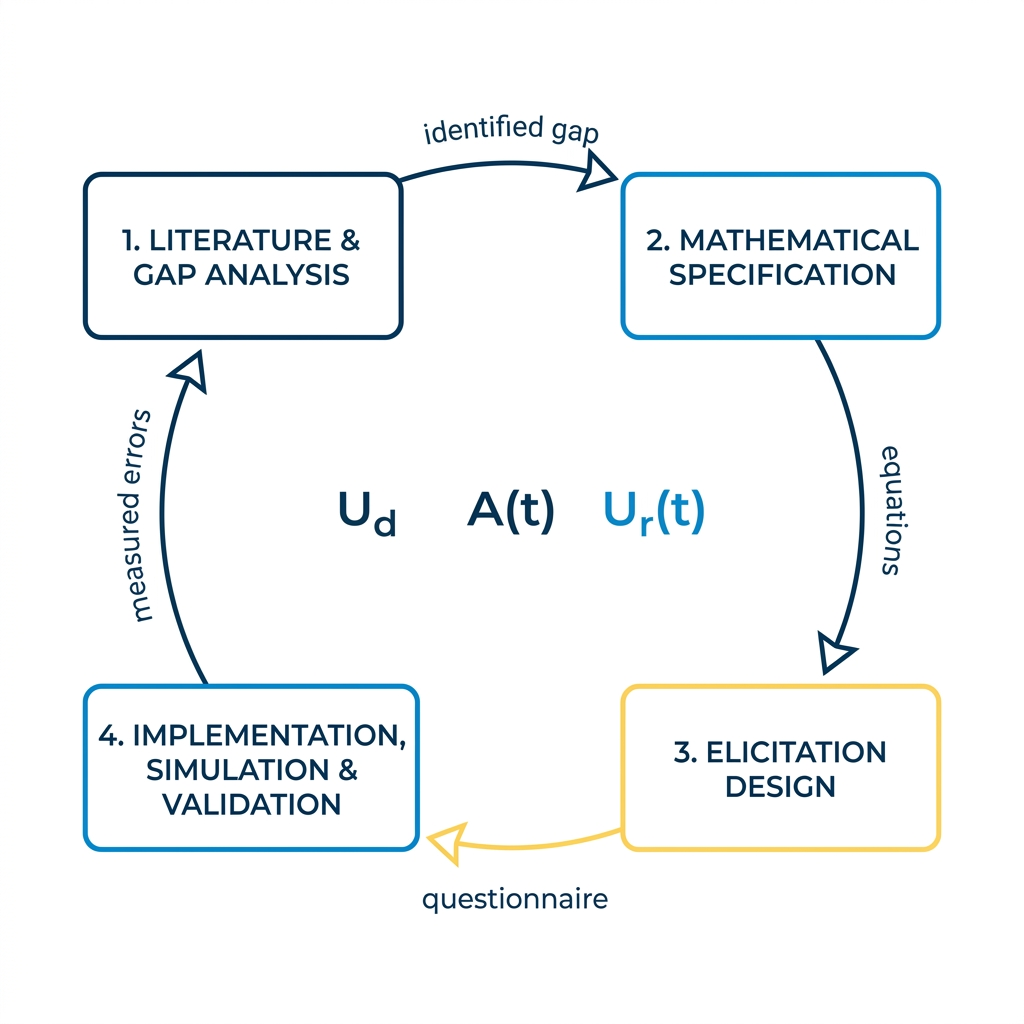
\includegraphics[width=0.72\linewidth]{Images/4.Operations/test_learn_loop.png}
    \caption{The test-and-learn iteration loop}
    \label{fig:testlearn}
\end{figure}

Figure~\ref{fig:testlearn} shows the loop as it was actually run. Each turn of it produced
either a working increment or a documented rejection, and the four rejections above are the
evidence that the second outcome was genuinely available rather than theoretical.

\paragraph{Quality gates.}
Agile without a definition of done produces velocity and nothing else. Three gates were
applied: no feature merged without automated tests, giving 1\,779 test functions at the end
of the mission; every business write passing through a single audited mutation service, so
that no result could be produced by an untraceable edit; and every reported figure
regenerated from raw artefacts by a script rather than transcribed by hand.

\subsection{Phases and Milestones}
\label{sec:planning}

The mission ran in six phases. Figure~\ref{fig:gantt} gives the schedule and
Table~\ref{tab:jalons} the milestones that closed each phase.

\begin{figure}[htbp]
    \centering
    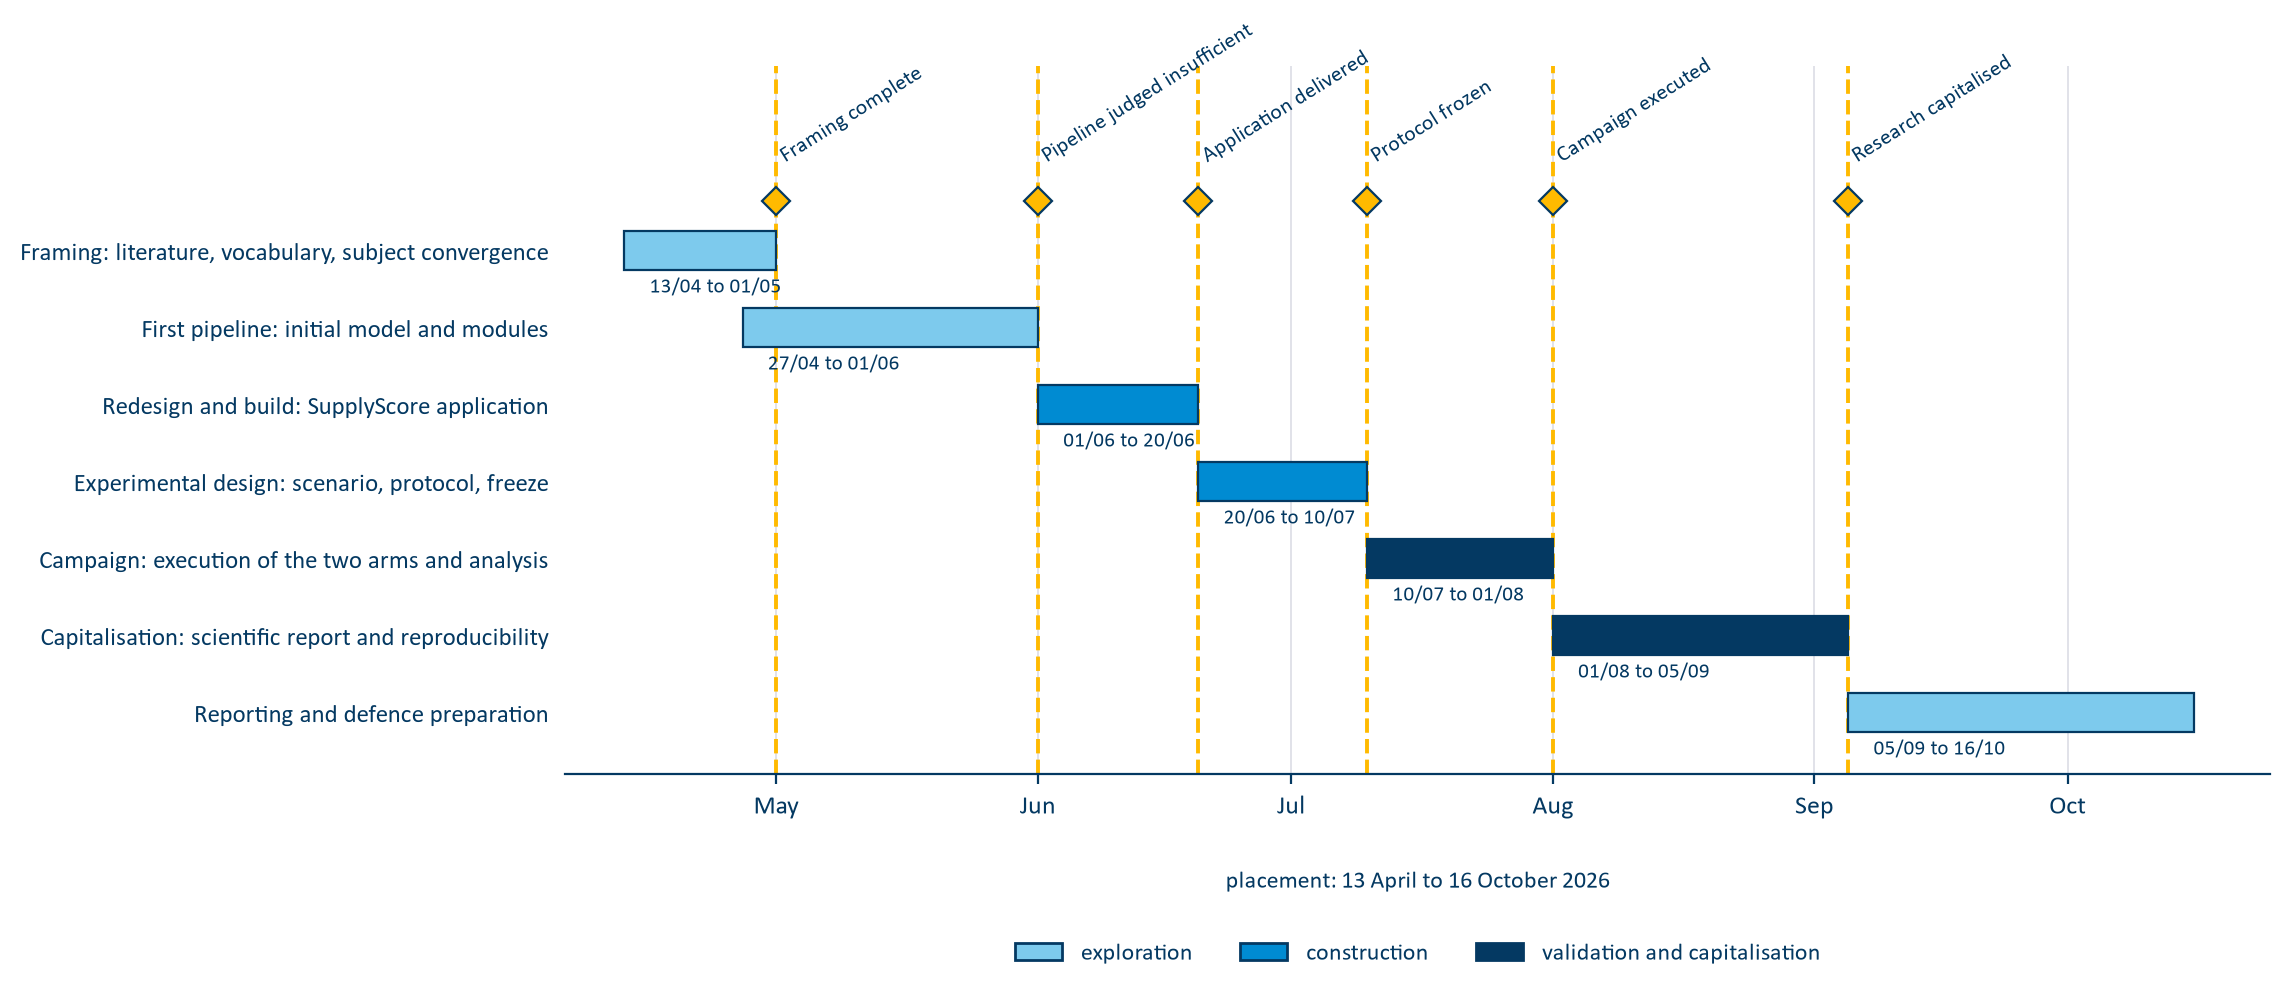
\includegraphics[width=0.96\linewidth]{Images/gantt.png}
    \caption{Phases and milestones of the mission}
    \label{fig:gantt}
\end{figure}

\begin{table}[htbp]
\centering
\caption{Milestones}
\label{tab:jalons}
\small
\begin{tabularx}{\linewidth}{>{\raggedright\arraybackslash}p{2.4cm} >{\raggedright\arraybackslash}p{3.4cm} X}
\toprule
\textbf{Date} & \textbf{Milestone} & \textbf{Closed by} \\
\midrule
End April & Framing complete & Knowledge transfer report and state of the art presented;
subject converged with the programme director \\
End May & First pipeline & End-to-end computation running, and found insufficient, which
triggered the redesign \\
Mid June & Application delivered & Multi-tenant persistence, audited writes, weekly cycle,
event engine, explainability, exports and backup \\
Early July & Protocol frozen & Scenario, data pack hashed, role cards and hypothesis
register registered before any data existed \\
End July & Campaign executed & Two arms run, analysed against the pre-registered register \\
Mid August & Research capitalised & Scientific report and reproducible derivation of every
figure \\
\bottomrule
\end{tabularx}
\end{table}

The planning was revised once, in June. The original schedule allocated the second half of
the mission to extending the model's scope; it was reallocated to validating what already
existed, on the argument that an unvalidated extension of an unvalidated model compounds the
problem rather than advancing it. That reallocation is the reason this report can state a
measured result at all.

\subsection{Risks and Mitigations}
\label{sec:risques}

Four risks were identified and carried at the start of the mission.
Table~
\ref{tab:risques} states each one, whether it materialised, and what was done about
it. Three of the four did materialise, which is a high rate and reflects how much of this
mission depended on things outside the author's control.

\begin{table}[htbp]
\centering
\caption{Risk register and outcomes}
\label{tab:risques}
\small
\begin{tabularx}{\linewidth}{>{\raggedright\arraybackslash}p{3.5cm} >{\raggedright\arraybackslash}p{1.8cm} X}
\toprule
\textbf{Risk} & \textbf{Outcome} & \textbf{Mitigation and effect} \\
\midrule
No access to academic literature from within ALTEN & Materialised & The Direction de
l'Innovation holds no journal or database subscriptions, so a state of the art conducted
from the company alone would have rested on whatever is publicly readable. The mission
depended throughout on ESTIA and Cranfield library credentials. It worked, but the
dependency is real and would block a consultant without a university affiliation. \\[3pt]
\midrule
Broad mission scope & Materialised & Five workstreams in the signed assignment against one
person and six months. Mitigated by converging the subject in the first weeks with the
programme director and recording the boundaries explicitly
(Section~\ref{sec:mission_perimetre}) rather than leaving them implicit. \\[3pt]
\midrule
Human campaign might not be securable & Materialised & Eight colleagues for nine working
days was never guaranteed. Mitigated by designing the protocol so that the declarant could
be substituted without changing the record format, which is what allowed the campaign to run
at all when the humans were unavailable. Cost: the external validity of every behavioural
claim. \\[3pt]
\midrule
CPU-only compute & Contained & No GPU available. Bounded model size and training resolution,
and is the reason one comparison was run at reduced scale. Mitigated by choosing methods
whose cost is dominated by data rather than by parameters. \\
\bottomrule
\end{tabularx}
\end{table}

The first risk deserves a comment, because it is the one least often written down. An R\&D
department that cannot read the literature it is meant to advance is dependent on the
academic affiliations of the people passing through it. For a placement holder on a double
degree that is invisible, since the credentials come with the student. It stops being
invisible the moment the work has to be continued by someone without them, which is a
succession risk for the programme rather than a problem for this mission.


\clearpage
\section{State of the Art}
\label{sec:etatdelart}
%% Consignes : « Incontournable pour le rapport de MFE, l'etat de l'art
%% presente les solutions techniques, methodes, outils, organisations
%% existants qui repondent pour tout ou en partie a la problematique posee.
%% Il s'agit de realiser une analyse critique des travaux existants. »

The question of Section~\ref{sec:question} touches several fields that do not usually cite
one another. This section reviews each for what it settles and, more importantly, for what it
leaves open. A structured evaluation of every source, recording its argument, method and
limitations, was maintained throughout the mission and informs the appraisals below.

\subsection{Deadline-Driven Value and Risk Propagation}

Real-time systems research models the value of a task as a function of when it completes.
Chen and M\"uhlethaler show that utility typically holds constant until a deadline and then
decreases~\autocite{cheng1996due}, and a wider survey confirms structured degradation past
critical thresholds~\autocite{cheng2025survey}. This establishes that urgency is legitimately
time-varying.

Separately, supply chain research formalises the ripple effect, whereby a local disruption
cascades through downstream tiers and amplifies as it
travels~\autocite{ivanov2020digital,ivanov2019viable,li2020exploring}. This establishes that
urgency is legitimately network-dependent.

\emph{Critical appraisal.} The first stream stops at a single isolated task and offers
nothing on combining heterogeneous indicators. The second models propagation but treats the
node-level score as given. Neither addresses a declared signal at all. Between them they
justify treating urgency as time-varying and propagated, and leave the aggregation question
entirely open.

\subsection{Indicators of Delivery Rupture}

If urgency is to be aggregated, the indicators must come from somewhere. Heckmann, Comes and
Nickel establish rupture as the terminal event a supply risk measure should anticipate, and
criticise the field for measuring exposure without connecting it to that
event~\autocite{heckmann2015critical}. Indicator-based supplier monitoring proceeds by
identifying observable precursors~\autocite{mokhtar2019supplier}.

Five families recur. Slack is the only indicator whose exhaustion is
irreversible~\autocite{cohen2021assigning,sun2020combating}. Capacity saturation adds waiting
time a nominal lead time does not
show~\autocite{tomlin2006value,hosseini2019resilient}. Resource performance is monitored
through composite proxies because supplier-side data is rarely
available~\autocite{mokhtar2019supplier,hlioui2017joint}. Adverse-event exposure is treated
probabilistically~\autocite{hosseini2020ripple,liu2021robust}. Cost signals are read as
symptoms of strain rather than causes~\autocite{shen2019managing}, and emissions constraints
restrict the admissible responses rather than causing
rupture~\autocite{hoen2014effect,smartfreight2023glec}.

\emph{Critical appraisal.} This literature names precursors and monitors them individually.
It supplies no criterion for deciding which belong in one composite, and says nothing about
whether equal numerical values on structurally different indicators carry equal risk meaning.
Both questions are inherited by any multi-block model, and
Section~\ref{sec:realisation_modele} treats the second explicitly.

\subsection{Cognitive Bias in Declared Urgency}

Zhu, Yang and Hsee report the mere-urgency effect across five controlled experiments:
participants consistently preferred imminent low-value tasks to distant high-value ones, and
the bias survived being told about it~\autocite{zhu2018mere}. Steel gives a formal
discounting model in which immediacy becomes more salient as a deadline
approaches~\autocite{steel2006integrating}. Field studies confirm the pattern under
workload~\autocite{rusou2020psychology,diwa2020task}.

\emph{Critical appraisal.} This stream diagnoses the problem and quantifies it in controlled
settings, but the magnitude in industrial supply chains is uncalibrated, and it prescribes no
operational correction. It justifies treating the declared signal as biased; it does not say
what to do about it.

\subsection{Multi-Criteria Elicitation and Aggregation}

Structured elicitation of a human judgment is a solved problem in outline. The Analytic
Hierarchy Process derives criteria weights from pairwise comparisons and validates them
through a consistency ratio~\autocite{saaty1980analytic}, though it is vulnerable to rank
reversal and to cognitive noise~\autocite{dyer1990,triantaphyllou2024}. The Best-Worst Method
reduces the number of comparisons required~\autocite{rezaei2015best}, and its fuzzy extension
absorbs judgment uncertainty~\autocite{guo2017fuzzy,liang2020}. For ranking alternatives
without letting a good score on one criterion mask a catastrophic one on another, outranking
methods such as PROMETHEE~II establish pairwise preference
flows~\autocite{brans1986promethee,behzadian2010promethee}.

The composite indicator literature supplies the necessary warning: nominal weights often
diverge from effective importance because of correlation and normalisation
effects~\autocite{greco2018,becker2017,borgonovo2021global}.

\emph{Critical appraisal.} These are static tools. They elicit and aggregate, and none is
routinely compared against a computed operational counterpart. The composite-index critique
is generally raised as a caveat at the end of a paper rather than turned into something a
running system checks on its own data.

\subsection{Digital Twins and Decision Support}

The digital twin concept was formalised by Grieves~\autocite{grieves2014digital} and extended
to manufacturing~\autocite{tao2018digital,fuller2020digital}. In supply chains it integrates
simulation, optimisation and machine learning~\autocite{ivanov2021digital}, with demonstrated
capability in disruption monitoring and
replanning~\autocite{ding2023realtime,leung2022digital,hrusovsky2021realtime}. Recent
human-in-the-loop cognitive twins capture human feedback to synchronise mental models with
simulated operations~\autocite{niloofar2023}.

\emph{Critical appraisal.} This is the family the delivered system belongs to, and the gap is
here. No retrieved system combines a declared urgency input, a computed operational urgency
and their propagated mismatch. A second gap matters for this mission specifically: these
systems are evaluated on how accurately they estimate physical state, and their inputs are
assumed to arrive. Where an input depends on the same operator whose judgment the system
exists to support, that circularity is not treated as a measurement problem.

\subsection{Verifying a Probabilistic Signal}

Because this mission scores a probabilistic signal against outcomes, it inherits forecast
verification. Brier introduced the mean squared error of probabilistic
forecasts~\autocite{brier1950verification}, and Murphy decomposed it into reliability,
resolution and uncertainty~\autocite{murphy1973vector}, establishing the distinction the
results of this report depend on: a forecast can order outcomes correctly while announcing
the wrong probabilities, and the two failures need different repairs. Machine learning
rediscovered the same point, finding strong classifiers that produce distorted probabilities
correctable by a cheap post-hoc layer~\autocite{niculescu2005predicting,guo2017calibration}.

\emph{Critical appraisal.} This literature assumes the outcome being predicted is
unambiguously defined. In an operational supply chain it is a modelling choice, and
Section~\ref{sec:realisation_resultats} measures that choice moving the reported result by a
factor of five.

\subsection{What the Review Establishes}
\label{sec:gap}

Each stream closes on a limit. Collected, those limits describe one absence rather than
several. The reviewed work covers multi-block risk aggregation, network propagation, digital
twin operation, multi-criteria elicitation and probabilistic verification. No retrieved work
combines them with a structured declared-urgency input and an empirical test of the resulting
adequacy signal against recorded outcomes.

That missing combination is what this mission set out to build and to test.


\clearpage
\section{Carrying Out the Mission}
\label{sec:realisation}
%% Consignes : « La presentation doit etre structuree autour de la demarche
%% de projet presentee precedemment. [...] Chaque fois que necessaire,
%% indiquer les productions. [...] Il est aussi pertinent d'indiquer les
%% problemes rencontres et les solutions ou strategies mises en oeuvre. »

This section follows the phases of Section~\ref{sec:planning}: the model, the system built
from it, the experiment designed to test it, what the experiment measured, and the problems
met along the way.

\subsection{The Model}
\label{sec:realisation_modele}

\subsubsection{Real urgency}

Real urgency is not read from a single deadline-proximity signal. It is aggregated at each
node from six indicator blocks selected from the literature of
Section~\ref{sec:etatdelart}: time, capacity, performance, risk, cost and carbon. Each
produces a partial urgency $u_m \in [0,1]$, and the aggregation is a weighted probabilistic
OR:

\begin{equation}
    U_{r,\text{local}} = 1 - \prod_{m} (1 - u_m)^{\omega_m}.
    \label{eq:ur}
\end{equation}

The choice of that form over a weighted average is the central modelling decision. A weighted
average is fully compensatory: a node with a completely failed capacity and healthy cost,
carbon and performance readings would score as moderately urgent. Equation~\ref{eq:ur} is
not: any block approaching its maximum drives the aggregate toward the maximum regardless of
the others. For a signal whose purpose is to catch the node that is about to fail,
non-compensatory behaviour is the required property.

\begin{table}[htbp]
\centering
\caption{The six indicator blocks and what each measures}
\label{tab:blocs}
\small
\begin{tabularx}{\linewidth}{>{\raggedright\arraybackslash}p{2.0cm} >{\raggedright\arraybackslash}p{2.7cm} X}
\toprule
\textbf{Block} & \textbf{Role} & \textbf{What it measures} \\
\midrule
Time & Direct cause & Probability that the realistic lead time exceeds the margin to the
next deadline. The only resource whose exhaustion cannot be reversed \\
Capacity & Direct cause & Saturation of storage, weight and throughput, which adds waiting
time a nominal lead time does not show \\
Performance & Direct cause & Drift in the productive health of the resource making the part,
through a composite availability, performance and quality proxy \\
Risk & Direct cause & Expected unavailability: failure probability times recovery time times
severity, revised weekly from declared events \\
Cost & Arbitration & Financial strain. Paying premium freight to protect a deadline is a
symptom, not a cause, and it bounds which responses stay affordable \\
Carbon & Arbitration & Emissions above target. Restricts the admissible set of responses,
typically in the sea-against-air trade-off \\
\bottomrule
\end{tabularx}
\end{table}

Table~\ref{tab:blocs} gives the six and separates them by role. Four describe a mechanism
that leads to rupture; two constrain which responses remain available once it threatens. Each
candidate indicator was screened against four questions before being retained: does it have a
plausible causal link to rupture, can it be measured or credibly estimated, can an operator
act on it, and does it add information the retained blocks do not already carry.
Figure~\ref{fig:blocs} draws the resulting structure.

\begin{figure}[htbp]
    \centering
    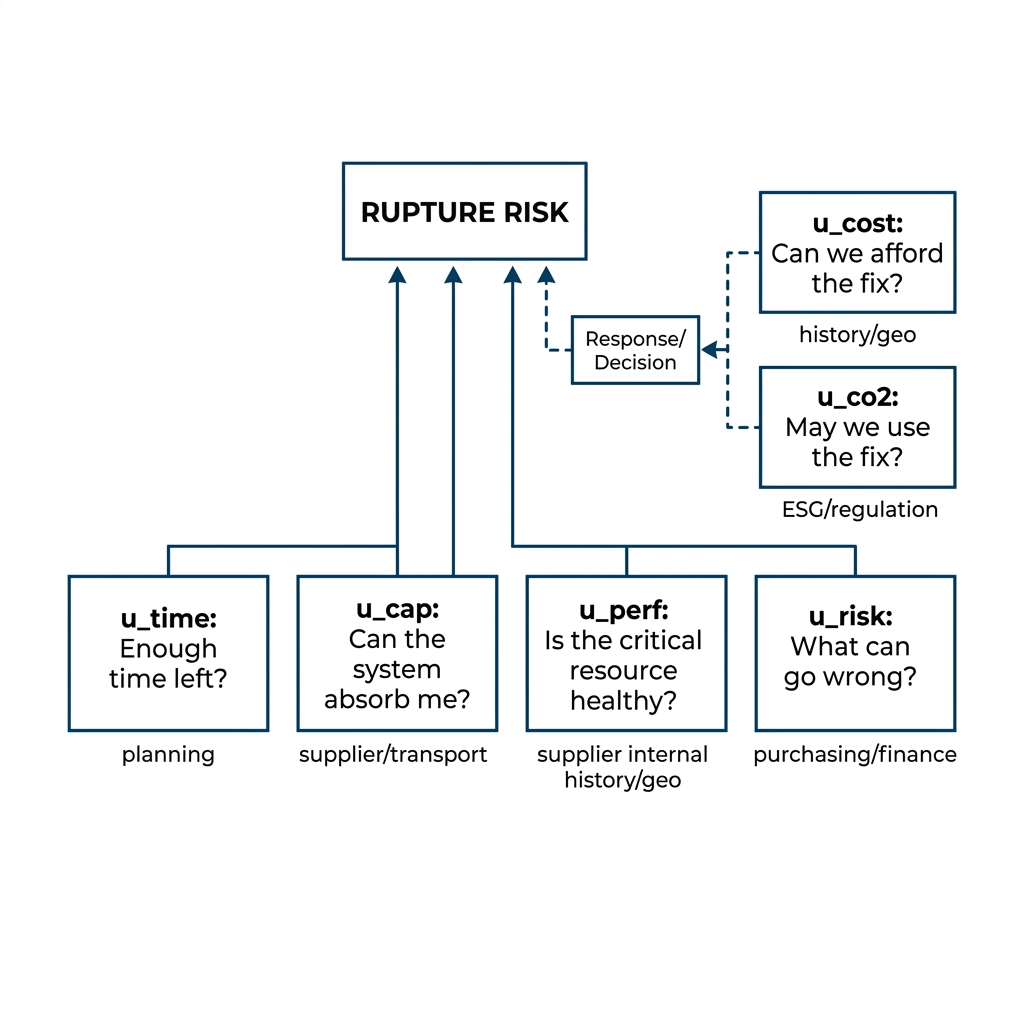
\includegraphics[width=0.80\linewidth]{Images/4.Operations/causal_tree_blocks.png}
    \caption{Causal structure behind the six-block selection}
    \label{fig:blocs}
\end{figure}

Three properties of that equation were specified explicitly, because a bare formula does not
state what its bounds mean. At $u_m = 0$ the block is nominal and its factor is $1$, leaving
the product unchanged. At $u_m = 1$ the factor is $0$ and the aggregate saturates. A block
whose data is unavailable is given weight $\omega_m = 0$, which is deliberately distinct from
$u_m = 0$: the first says nothing is known, the second asserts the block is healthy.

\paragraph{The assumption that the blocks are exchangeable.}
The product is symmetric in its factors, so it treats the six blocks as interchangeable up to
their weights. That does not hold cleanly. A value of $u_{\text{time}} = 0.3$ is a
probability of missing a deadline; $u_{\text{cost}} = 0.3$ is an ordinal position on a
normalising scale wearing a cardinal number. They are not equally informative about rupture.
The consequence was carried rather than hidden: the aggregate is used for ranking and for
comparison against the declared value, never as a calibrated probability in its own right.

\subsubsection{Declared urgency and the adequacy score}

Declared urgency is not collected as a free-text estimate. At each node the operator compares
four criteria pairwise through AHP, which yields a consistency-checked weight per criterion,
then rates each on a severity scale. The four criteria were chosen so that each has a
computed counterpart: operational impact and downstream dependencies mirror the severity the
propagation amplifies, the time window mirrors the time block, and recoverability mirrors the
recovery term of the risk block. Without that correspondence the later comparison would be
between unrelated quantities.

\begin{figure}[htbp]
    \centering
    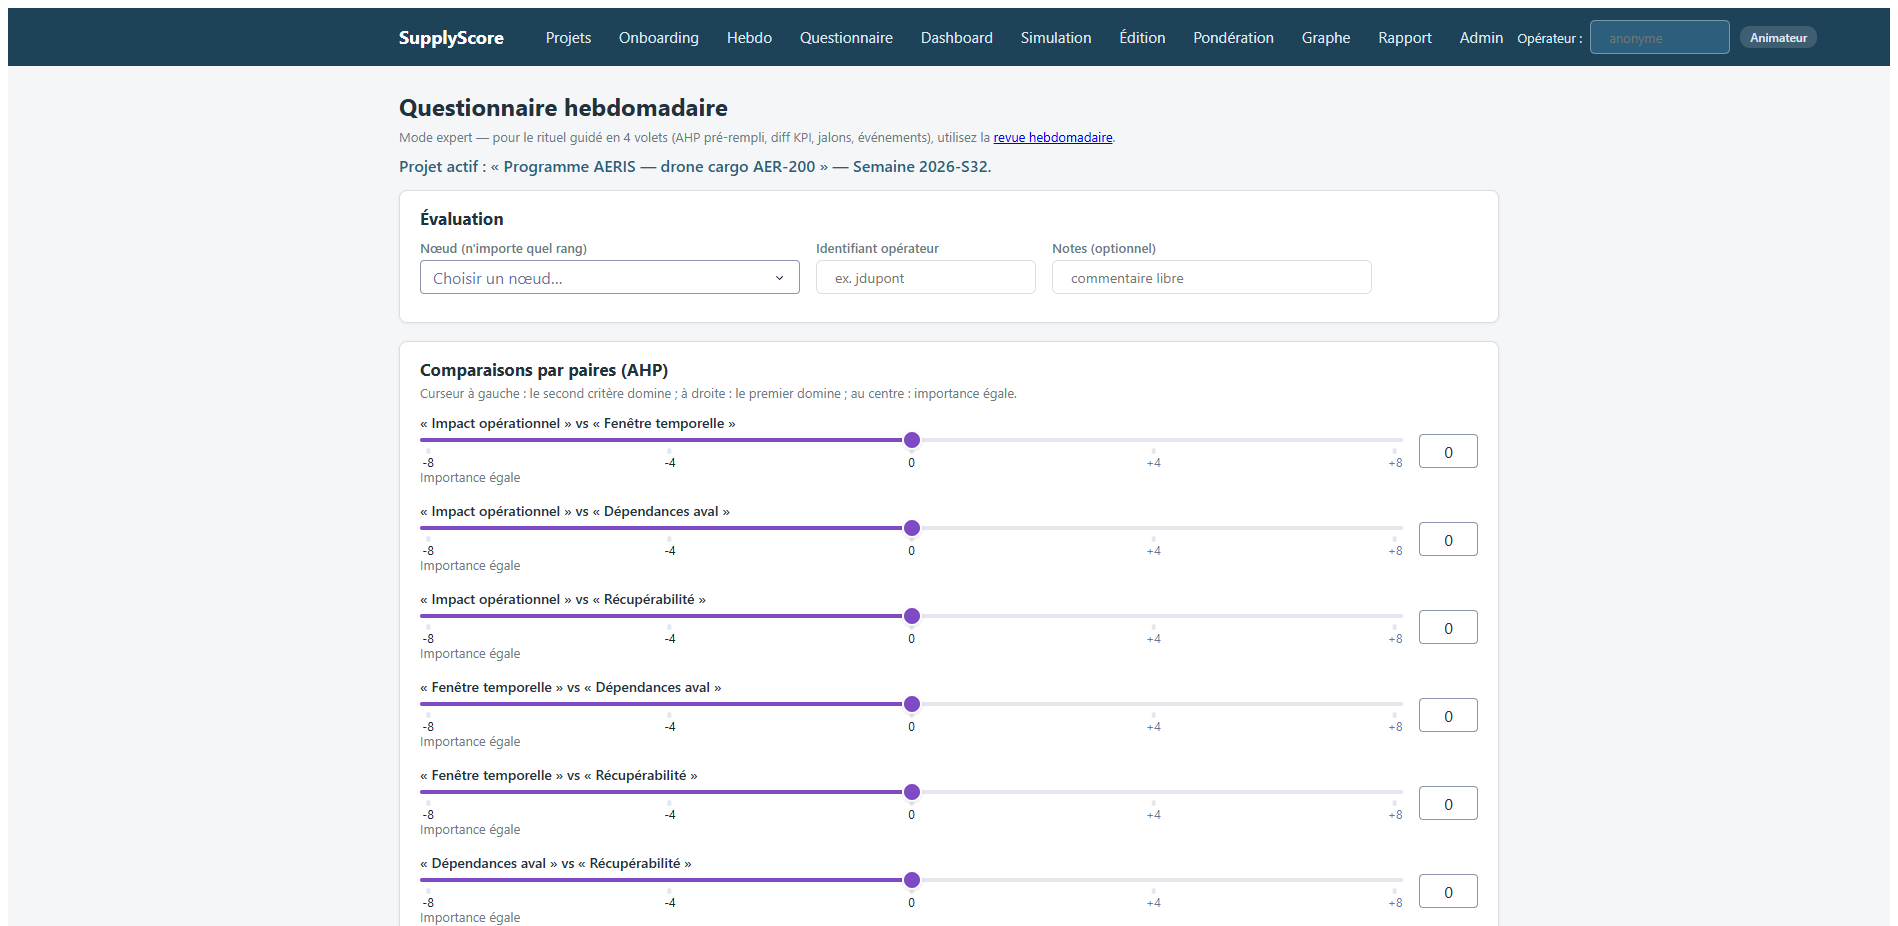
\includegraphics[width=0.76\linewidth]{Images/4.Operations/questionnaire_screenshot.png}
    \caption{The pairwise comparison questionnaire and its consistency gate}
    \label{fig:questionnaire}
\end{figure}

Figure~\ref{fig:questionnaire} shows the questionnaire as the operator meets it. A weight
vector whose consistency ratio exceeds the accepted threshold is refused, and the operator is
sent back to the most contradictory of their own comparisons before the assessment can enter
the network. Without that gate an incoherent judgment would propagate as though it were a
considered one.

Both signals then propagate across the supplier network, and in opposite directions: declared
urgency descends from the customer toward suppliers, real risk ascends from suppliers toward
the customer. The asymmetry is deliberate. Demand pressure is something a customer transmits
to its suppliers; physical risk is something suppliers transmit to their customer. A model
that propagated both the same way would be describing neither.

Figure~\ref{fig:propagation} shows the two signals travelling in opposite directions across
the same graph.

\begin{figure}[htbp]
    \centering
    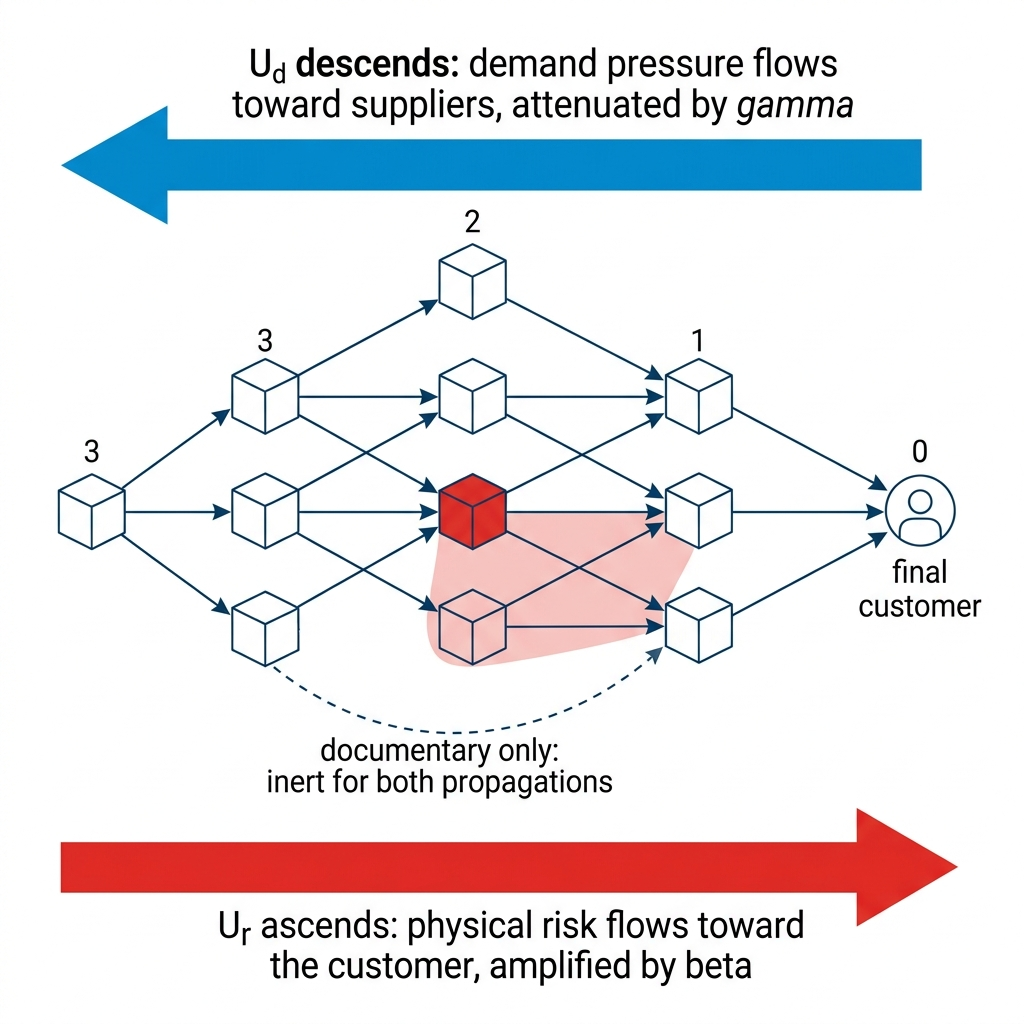
\includegraphics[width=0.80\linewidth]{Images/4.Operations/urgency_propagation.png}
    \caption{Bidirectional propagation across the supply network}
    \label{fig:propagation}
\end{figure}

Their mismatch, once both are propagated, splits into two named pathologies: false urgency
where the declaration exceeds the state, hidden risk where the state exceeds the declaration.
It is scored on $[0,100]$ through an asymmetric penalty that prices hidden risk at roughly
twice false urgency, following the clinical principle of Section~\ref{sec:pourquoi}.

\begin{figure}[htbp]
    \centering
    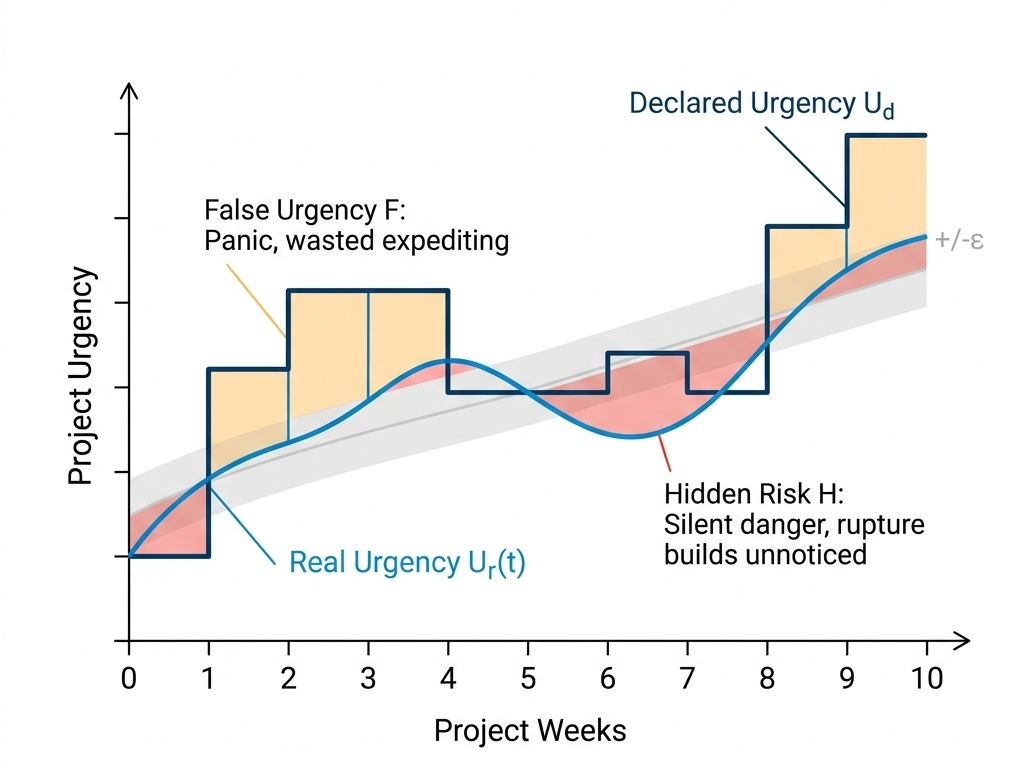
\includegraphics[width=0.80\linewidth]{Images/2.Problem/urgency_gap.png}
    \caption{Declared and real urgency, and the two mismatch pathologies}
    \label{fig:gap}
\end{figure}

Figure~\ref{fig:gap} shows the two signals over the life of a task. The step line is the
declaration, which moves only when a review is submitted; the smooth curve is the computed
state, which moves continuously. Where the step line sits above the curve the enclosed area
is false urgency; where the curve sits above the step line it is hidden risk.

\subsection{The System}
\label{sec:realisation_systeme}

The model was delivered as SupplyScore, a standalone Python application of 73 modules across
10 packages, covered by 1\,779 automated test functions in 106 test files, driving a
multi-page web interface over a per-node database layer.

Four architectural decisions carry the engineering weight. Every operation passes through a
single orchestrating facade, so there is no second write path. Data is split into one
registry database plus one database per node, which enforces that one supplier's history is
not readable through another's. Every business write crosses a single mutation service that
validates ranges, diffs against current state and records the change with its author, making
the audit trail a property of the architecture rather than a convention. And each project
carries its own clock, which is what allows a six-month scenario to be replayed in
compressed time without touching the model.

\begin{figure}[htbp]
    \centering
    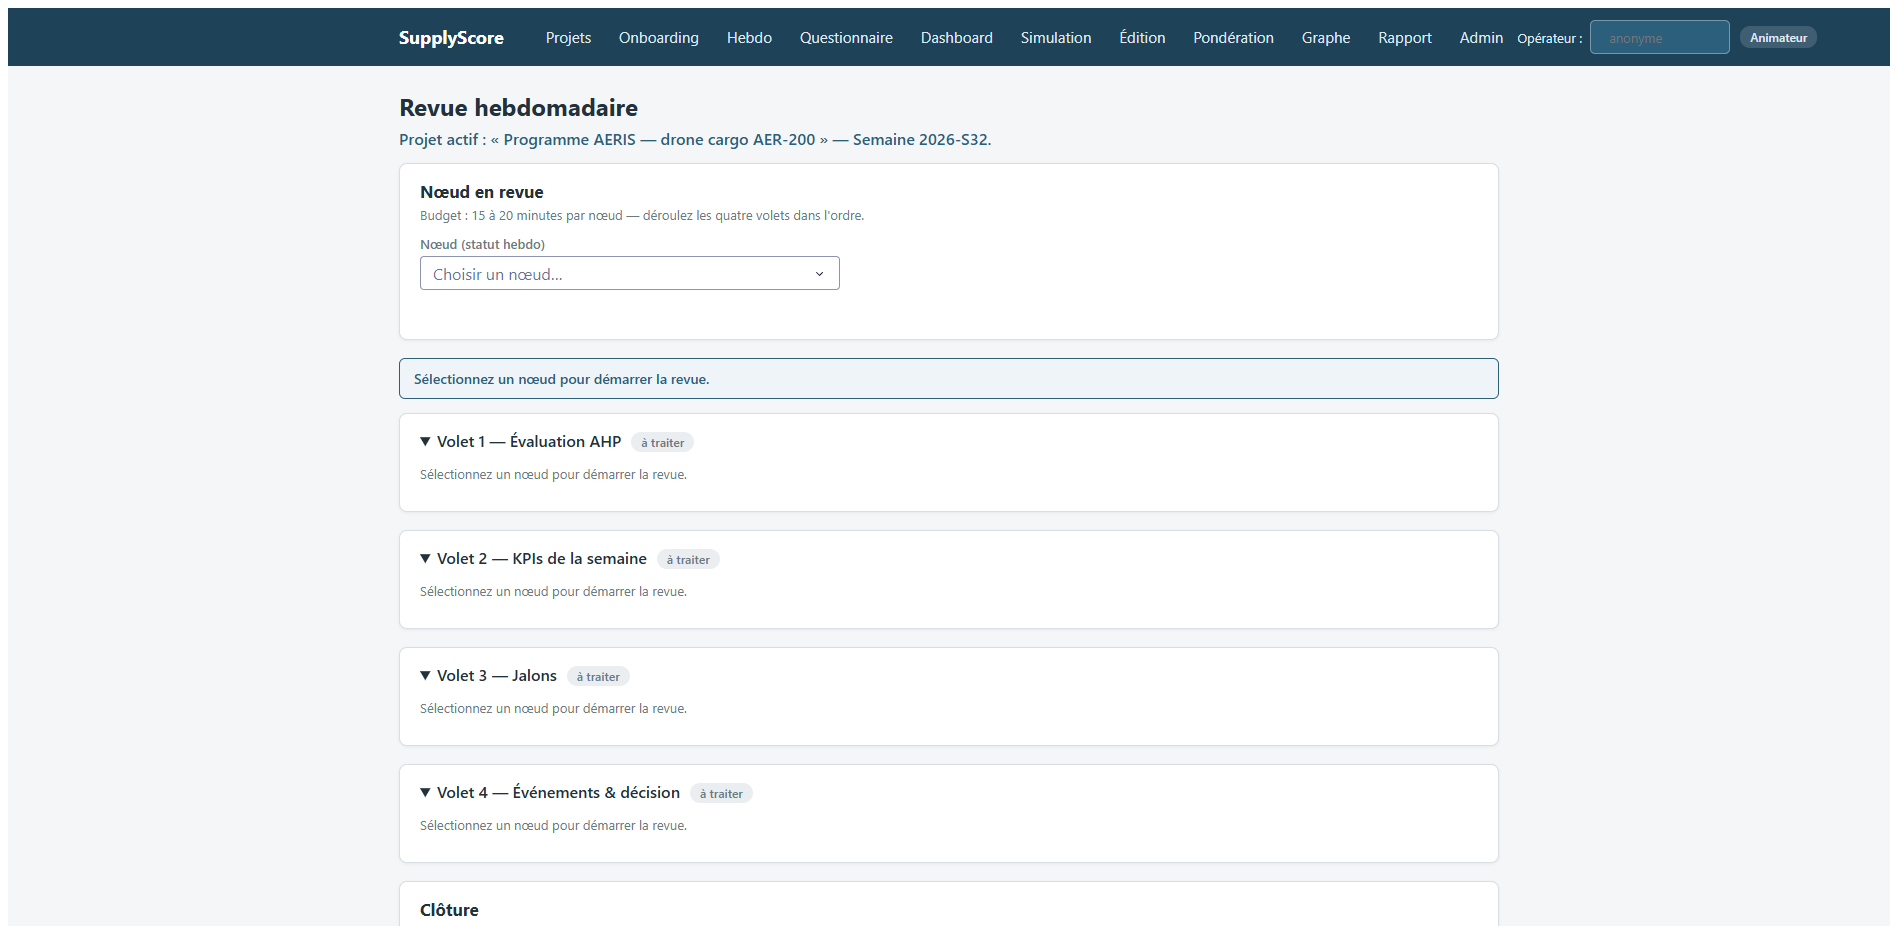
\includegraphics[width=0.76\linewidth]{Images/4.Operations/hebdo.png}
    \caption{The weekly review page}
    \label{fig:hebdo}
\end{figure}

Figure~\ref{fig:hebdo} shows the operator's main entry point. Its four sections, the
questionnaire, the week's indicator values, milestone progress and any events, commit as a
single signed transaction so that no partial review can enter a node's history.

\begin{figure}[htbp]
    \centering
    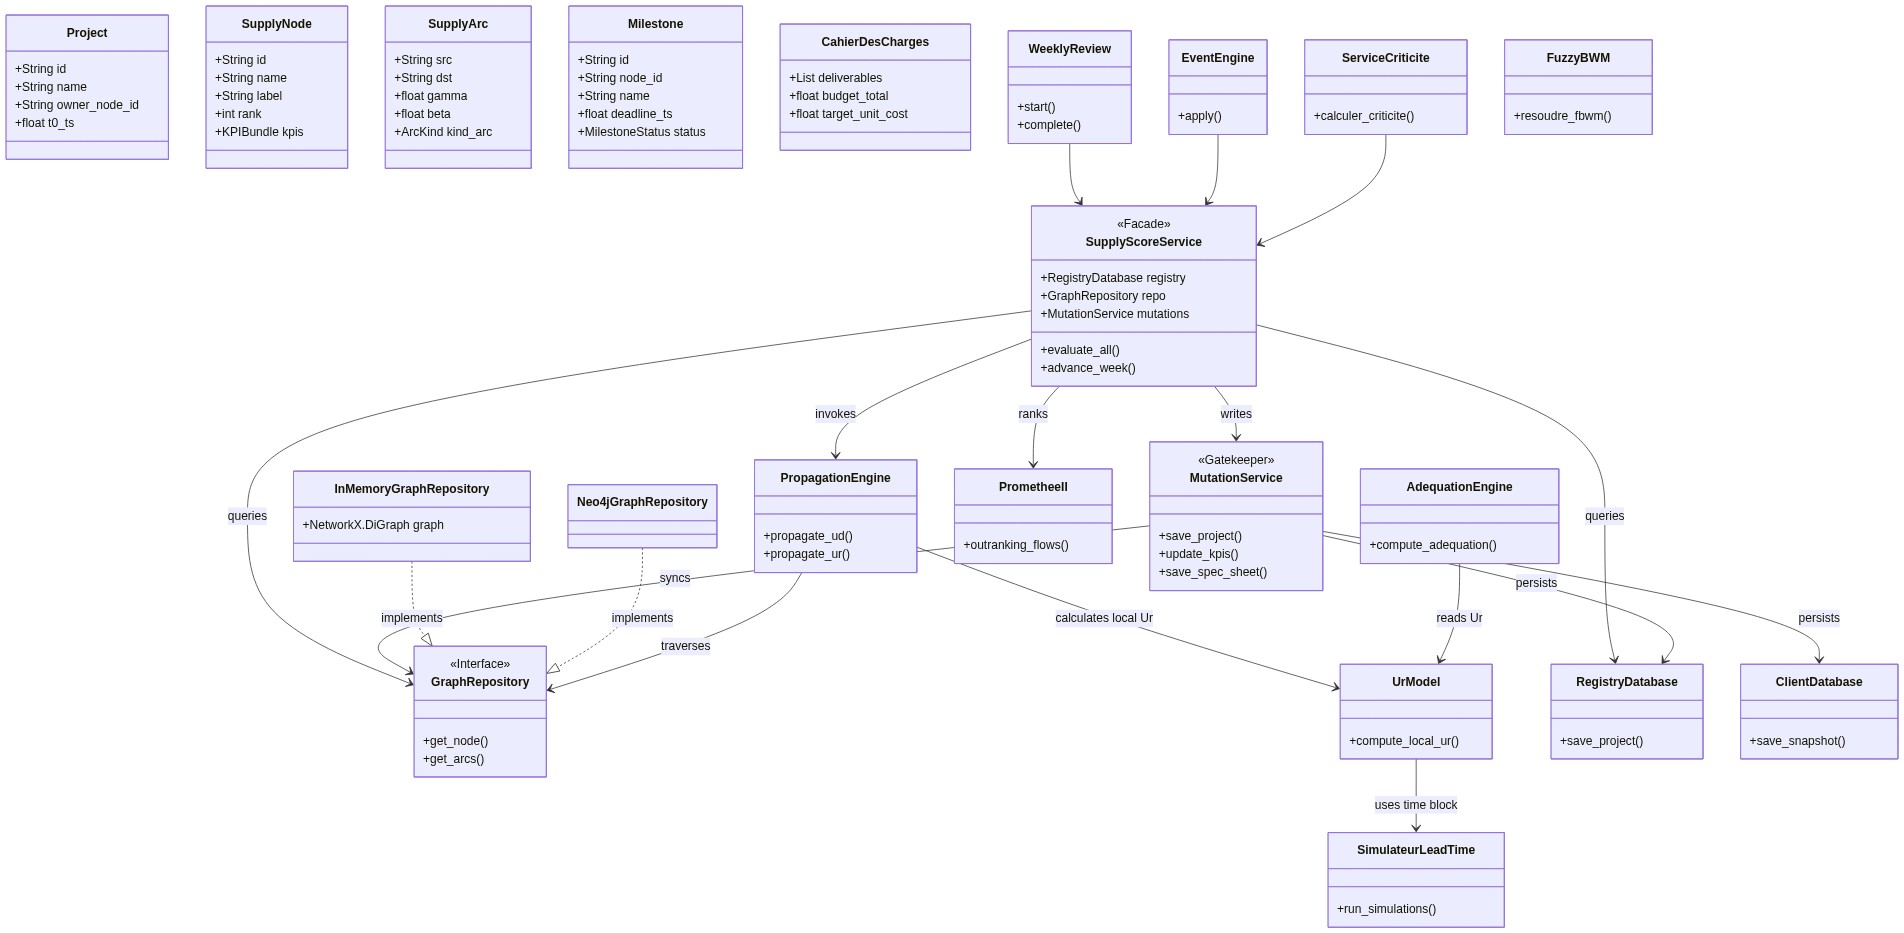
\includegraphics[width=0.74\linewidth]{Images/4.Operations/uml_architecture.png}
    \caption{System architecture: single facade, audited writes, per-node persistence}
    \label{fig:archi}
\end{figure}

Figure~\ref{fig:archi} shows how those pieces relate. The single entry point is what makes
the audit guarantee enforceable rather than aspirational: there is no path into the data that
bypasses it, including from the administration interface.

Two capabilities proved more important than anticipated. The explainability page reconstructs
any score term by term, decomposing the declared value into one contribution per criterion
and the computed value into one per block, so that a coordinator asking why a node scored as
it did receives an exact answer rather than a plausible one
(Figure~\ref{fig:explain}). That is what made the diagnosis in
Section~\ref{sec:realisation_resultats} possible from the application rather than by hand.
The export produces frozen data for analysis outside the tool, which the whole experimental
analysis relies on.

\begin{figure}[htbp]
    \centering
    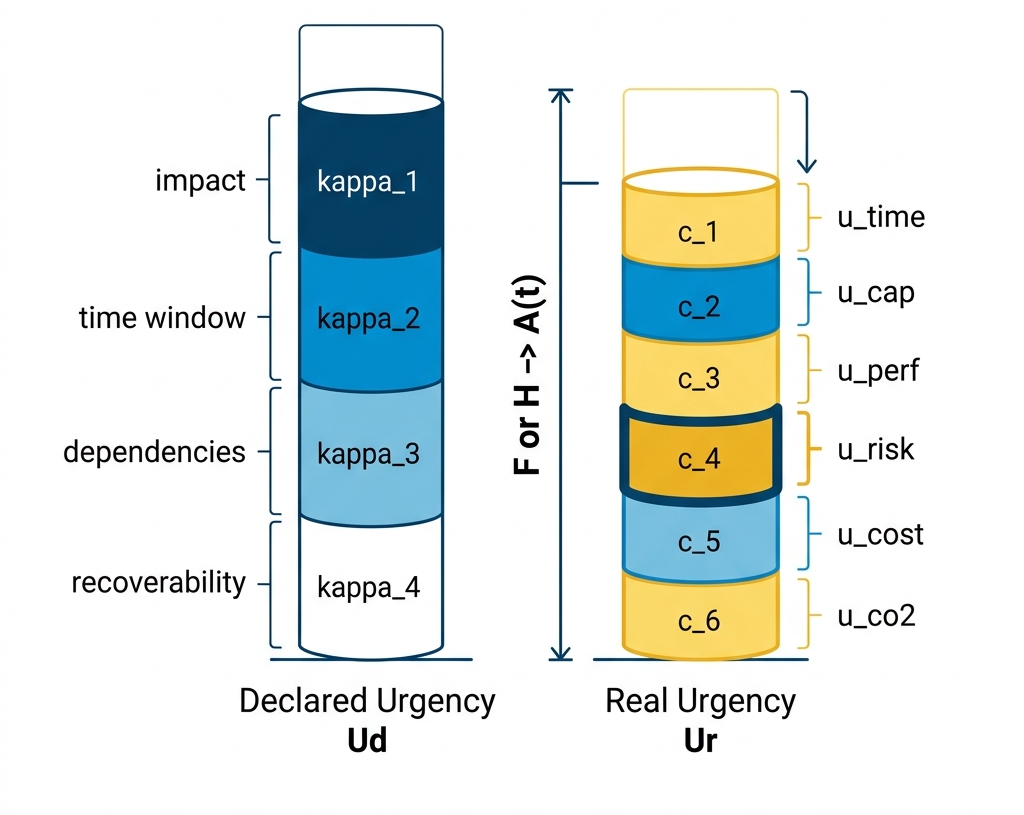
\includegraphics[width=0.78\linewidth]{Images/4.Operations/explainability_waterfall.png}
    \caption{Per-node explainability: exact decomposition of both signals}
    \label{fig:explain}
\end{figure}

\subsection{The Experiment}
\label{sec:realisation_experience}

Building a system that computes a number establishes nothing about whether the number means
anything. The mission therefore included an experiment designed before the system was
finished.

The campaign replays the 2020 to 2022 semiconductor shortage over nineteen turns across an
eight-node satellite supply chain, from a raw wafer supplier through a foundry, a
distributor, a freight operator and an electronics manufacturer to the satellite prime. Real
urgency is fed from public time series of the actual crisis; declared urgency comes from the
participants through the weekly questionnaire. The two signals therefore have independent
sources, which is the precondition for the gap between them to mean anything.

\begin{figure}[htbp]
    \centering
    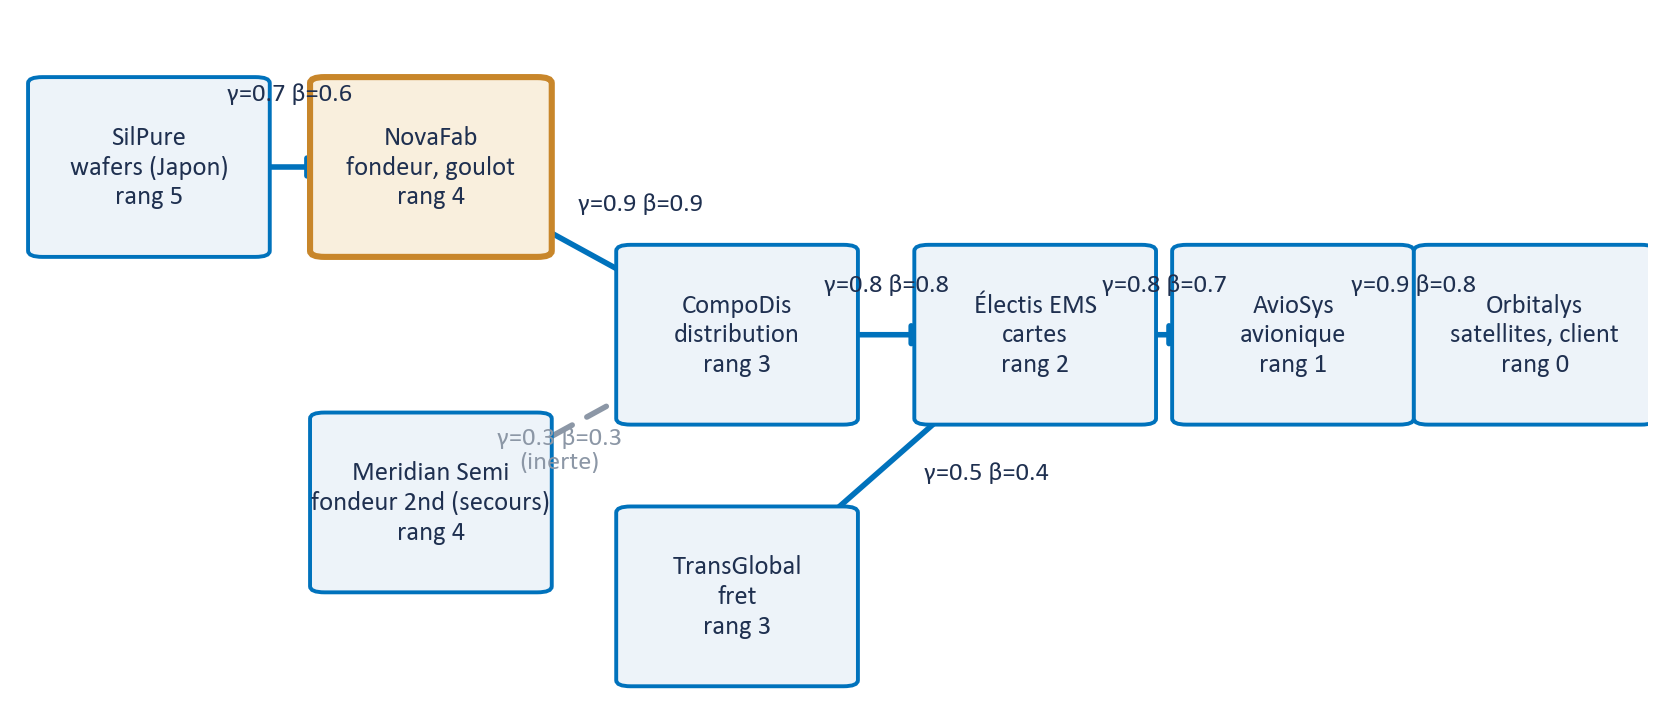
\includegraphics[width=0.94\linewidth]{Images/4.Operations/helios_network_coefficients.png}
    \caption{The campaign network and its per-arc coefficients}
    \label{fig:reseau}
\end{figure}

Figure~\ref{fig:reseau} gives the network, with the coefficient attenuating demand as it
descends and the one amplifying risk as it ascends, and each node's tier. The foundry at the
deepest tier is the expected bottleneck. The dashed arc into the secondary foundry is
deliberately inert: it represents the announced alternative supplier that in the real crisis
had no spare capacity, and modelling it as present but carrying nothing is the point.

Four artefacts were frozen before any data existed: the scenario with its twelve calibrated
events, the data pack with a hash recorded per file, the role cards, and a register of six
hypotheses each carrying a numeric threshold. Freezing the thresholds in advance is what
prevents a disappointing result from being rescued by moving the bar afterwards.

The design compares two arms on the identical frozen scenario. In the control arm, eight
isolated declarants each see only their own role card and turn briefing and declare blind. In
the treatment arm, the same declarants are additionally shown the system's own predictive
analysis of their node before declaring, and record whether it influenced them. Because the
scenario is frozen, the forecasts are identical between arms, so any behavioural difference
belongs to the act of displaying them.

\subsection{Results}
\label{sec:realisation_resultats}

\subsubsection{The signal does not predict outcomes}

Scored against the outcome definition the system itself applies, meaning a missed milestone,
an abandoned node or a critical event within four weeks, the forecast layer fails on both
axes that matter.

Discrimination is indistinguishable from chance: the area under the ROC curve ranges from
$0.37$ to $0.56$ across horizons and every confidence interval contains $0.5$. That statement
carries a caveat, since the positive class holds between two and six observations, which is
too few to conclude in either direction.

Calibration fails much more clearly, and does not depend on that small sample. The Brier
skill against a forecaster that simply announces the base rate is between $-3.4$ and $-6.9$,
meaning the model is several times worse than the trivial baseline.
Table~\ref{tab:fiabilite} localises the failure.

\begin{table}[htbp]
\centering
\caption{Reliability of the four-week forecast}
\label{tab:fiabilite}
\small
\begin{tabularx}{\linewidth}{l >{\centering\arraybackslash}X >{\centering\arraybackslash}X >{\centering\arraybackslash}X >{\raggedright\arraybackslash}p{3.6cm}}
\toprule
\textbf{Announced band} & \textbf{$n$} & \textbf{Mean announced} & \textbf{Observed} &
\textbf{Reading} \\
\midrule
$[0.0,\ 0.1)$ & 74 & 0.070 & 0.081 & Well calibrated \\
$[0.1,\ 0.2)$ & 24 & 0.128 & 0.000 & None materialised \\
$[0.2,\ 0.5)$ & 1  & 0.354 & 0.000 & None materialised \\
$[0.5,\ 0.9)$ & 7  & 0.859 & 0.000 & None materialised \\
$[0.9,\ 1.0]$ & 14 & 0.992 & 0.000 & None materialised \\
\bottomrule
\end{tabularx}
\end{table}

The pattern is unambiguous, and Figure~\ref{fig:fiabilite} shows it, with each marker's area
proportional to the number of forecasts in its band and the diagonal marking perfect
calibration. Where the model announces a low probability it is right: 74 forecasts averaging
$0.070$ were followed by an adverse outcome $8.1\%$ of the time. Where it announces a high
probability it is wrong every time: twenty-one forecasts announcing a mean of $0.948$ were
followed by the predicted outcome zero times.

\begin{figure}[htbp]
    \centering
    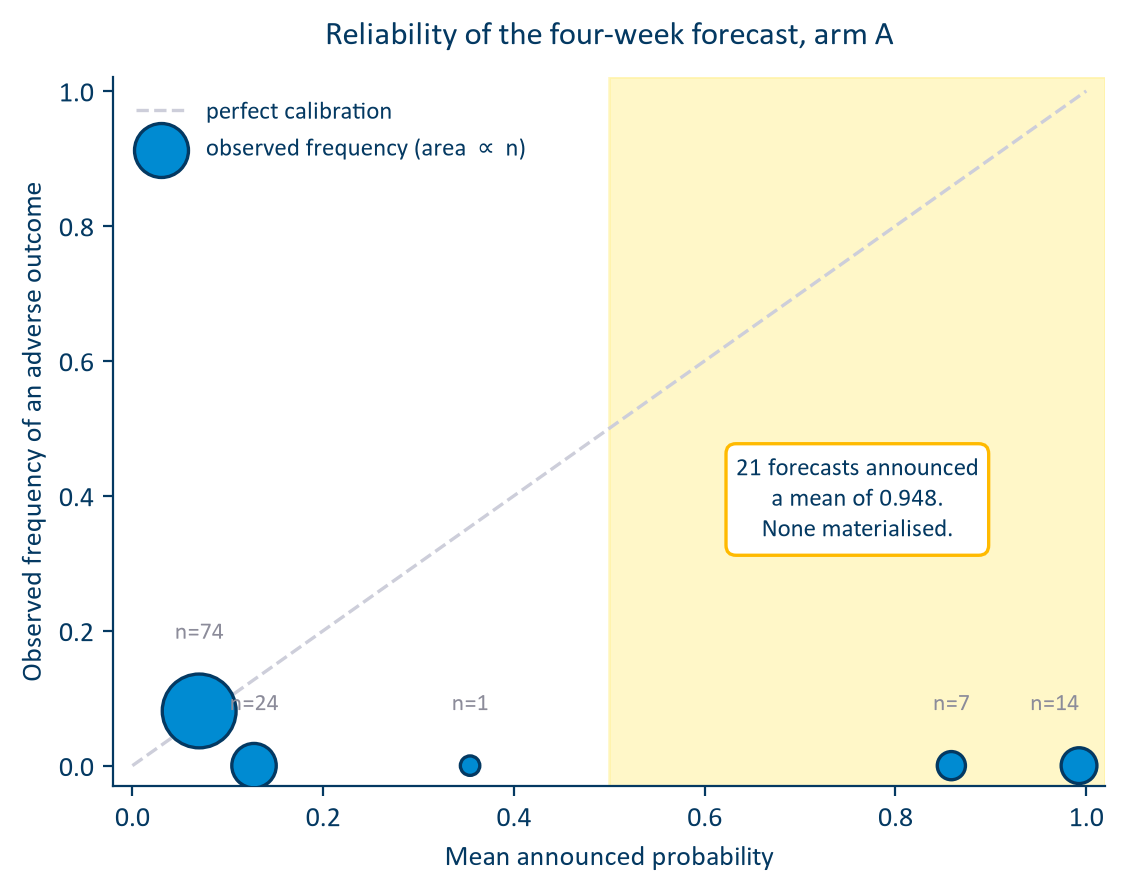
\includegraphics[width=0.84\linewidth]{Images/armA_reliability.png}
    \caption{Reliability of the four-week forecast}
    \label{fig:fiabilite}
\end{figure}

Separating these two failures matters for what happens next, and it is the distinction Murphy
established for exactly this purpose~\autocite{murphy1973vector}. A forecast that orders
outcomes correctly but announces the wrong numbers is repaired by a thin post-hoc layer that
leaves the model untouched. A forecast that does not order outcomes at all needs the model
changed. On this campaign the evidence for the second is weak, resting on very few positive
observations, while the evidence for the first is strong and does not depend on that sample
at all.

\subsubsection{Why: one block explains all of it}

The explainability layer localised the cause. Across all twenty-one confident forecasts, the
four-week probability and the milestone-miss probability never differ by more than $0.020$:
the confident tail is the milestone channel and nothing else. Set against the registry, ten
of the eighteen campaign milestones completed, eight remained active and only one was
actually missed. The model announced near-certain misses for six nodes that all delivered.

Reading the time block directly at the turn the scenario's critical event lands confirms it
from the other side: the block reads numerically zero at six of the eight nodes in the middle
of a crisis. The cause is structural. The block computes milestone risk from a lead-time
distribution against a deadline, while the event engine writes to capacity, cost and failure
probability and never to lead time. No path connects a shock to the quantity the block reads,
so the block cannot respond to a disruption. It is blind by construction, and because it
drives the entire confident tail, so is the forecast.

This is a defect in the model rather than a property of the scenario. Any deployment would
inherit it, and the repair is a change to the event mapping rather than to the mathematics.
It is the single most actionable finding of the mission.

\subsubsection{What happens when the forecast is shown to the operator}

The treatment arm produced a second result, and one that was not sought.

For the first four turns the forecast is hidden and all eight declarants record no influence.
At the turn it first becomes visible, all eight record one, and the direction is entirely
one-sided: five revised their declared urgency downward and three had their existing
assessment confirmed. Not one revised upward. The first upward revision anywhere appears the
following turn, and the scenario's single critical event lands two turns after the moment
every declarant was either reassured or confirmed.

\begin{figure}[htbp]
    \centering
    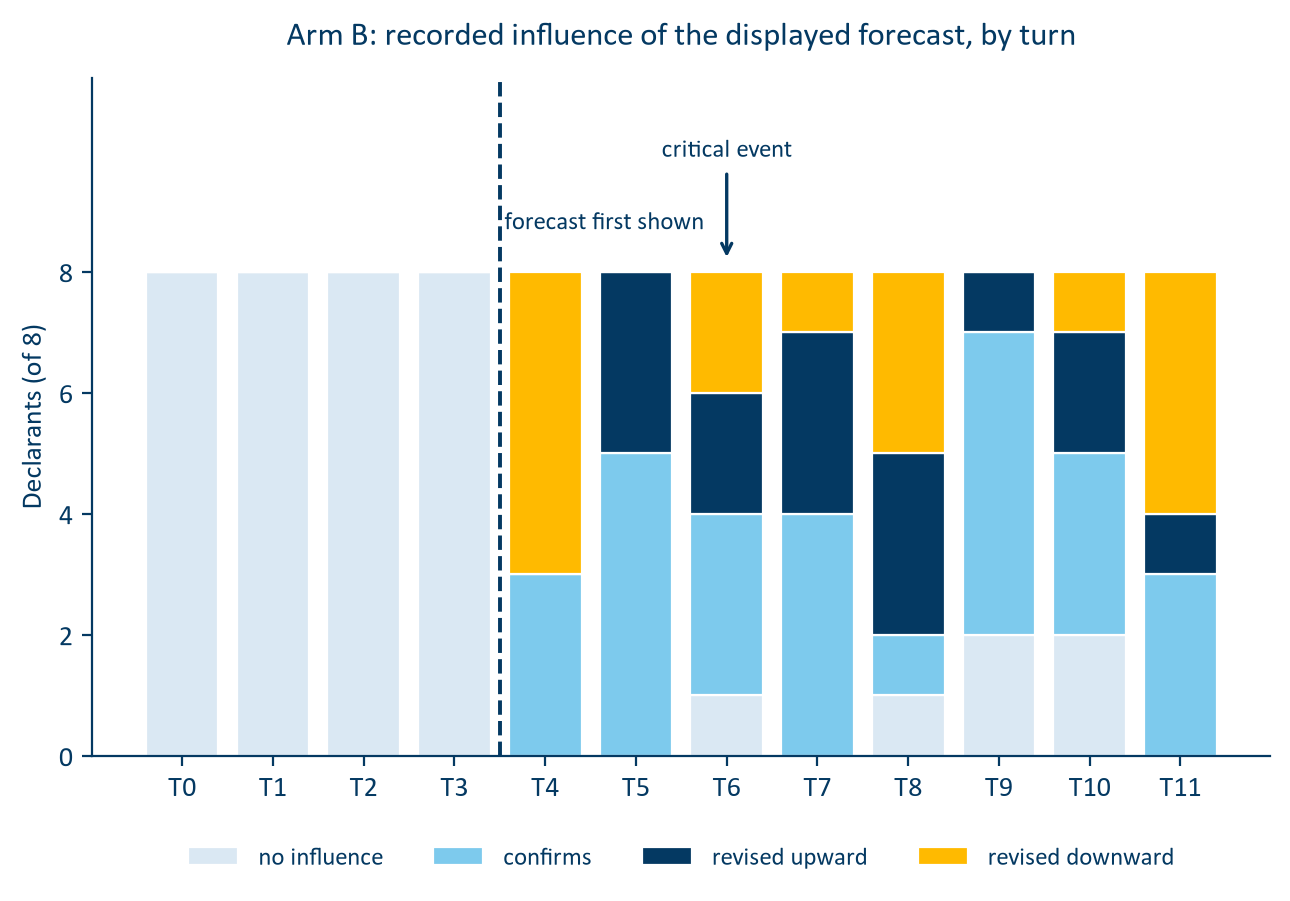
\includegraphics[width=0.90\linewidth]{Images/armB_influence.png}
    \caption{Influence of the displayed forecast, by turn}
    \label{fig:armB}
\end{figure}

Figure~\ref{fig:armB} shows the distribution turn by turn. Over the full campaign the balance
is close to even, 15 upward against 16 downward, so the one-sided effect belongs to first
contact rather than being a permanent bias.

Two things make this worse than a curiosity. The forecast being displayed comes from the same
layer whose confident predictions never materialise, and whose time block is blind to the
very shock about to arrive. And it is displayed as a numeric probability with a confidence
interval, a format the automation-bias literature identifies as increasing
reliance~\autocite{goddard2012automation,bansal2021whole}. The system was presenting an
unfounded reassurance in its most persuasive available form, immediately before the event it
had failed to anticipate.

One qualification cuts against the strongest reading: the recorded field captures the effect
on the declared level, not on the action taken, and the free-text notes show declarants still
acting protectively. The effect is on the measurement, which is nonetheless the input the
whole adequacy layer consumes.

\subsubsection{The outcome definition moves the answer}

A final measurement concerns how these results should be read at all. Scoring the identical
forecasts against a plausible but naive outcome definition, counting any recorded event
rather than the production definition, moves the base rate from $5.0\%$ to $38.7\%$ and
improves the apparent Brier skill from $-3.36$ to $-0.64$, while leaving discrimination
essentially unchanged.

The model did not change. Only the definition of truth did. An analyst choosing the easier
target would report a system five times better calibrated without a line of code being
touched. A calibration figure quoted without its outcome definition therefore carries little
information, which is a methodological result worth more to the programme than the score
itself.

\subsection{Problems Encountered and How They Were Resolved}
\label{sec:problemes}

Four difficulties shaped the mission, beyond the risks of Section~\ref{sec:risques}.

\paragraph{The first model could not represent the problem.}
The initial formulation expressed urgency as a single time-driven curve. It could not
represent a node on schedule but out of capacity, which is a common and dangerous state. The
resolution was to abandon it in April in favour of multi-block aggregation. The cost was
roughly three weeks; the alternative was building a validated implementation of an
inadequate model.

\paragraph{Measuring the gap requires two independent signals, which is harder than it looks.}
The same difficulty recurred three times in different disguises. A first synthetic dry run
derived the declared value from the computed one, so no gap could appear. The blind arm used
declarants who read their briefings so carefully that their declaration reproduced the
computed state. The treatment arm closed the loop deliberately by showing the model's output
to the declarant. Each time the symptom looked like a modelling problem and each time the
cause was circularity in the measurement. The resolution was to state the independence
requirement as a first-class design constraint and to record, for every result, which of the
two signals could have contaminated the other.

\paragraph{The literature was not accessible from inside the company.}
As set out in Section~\ref{sec:risques}, ALTEN's Direction de l'Innovation holds no journal or
database subscriptions. The state of the art was built entirely on ESTIA and Cranfield
library access. The practical resolution was to front-load literature retrieval into the first
weeks while planning which sources would be needed later, since retrieving a paper was never
a same-hour operation.

\paragraph{Compute was limited to a CPU.}
No GPU was available. This bounded what could be attempted and is the reason one comparison
was run at reduced scale. The resolution was methodological rather than material: choosing
approaches whose cost is dominated by the quantity of data rather than by model size, and
accepting the reduced scale explicitly in the reporting instead of quietly omitting the
comparison.


\clearpage
\section{Conclusion and Personal Assessment}
\label{sec:conclusion}
%% Consignes : « Toujours tres importante, la conclusion comporte : une
%% appreciation qualitative et quantitative des resultats et de l'avancement
%% du projet [...] des perspectives [...] un bilan personnel [...] Il est en
%% particulier demande a l'eleve de faire le lien avec le referentiel de
%% competences de l'ingenieur ESTIA. »

\subsection{Results Against the Objectives}
\label{sec:conclusion_objectifs}

Table~\ref{tab:bilan} assesses each objective of Section~\ref{sec:objectifs} against its
indicator. Four of five were met. The fifth was answered, and the answer was negative.

\begin{table}[htbp]
\centering
\caption{Objectives against outcomes}
\label{tab:bilan}
\small
\begin{tabularx}{\linewidth}{>{\raggedright\arraybackslash}p{0.7cm} >{\raggedright\arraybackslash}p{2.4cm} X}
\toprule
& \textbf{Status} & \textbf{Evidence} \\
\midrule
O1 & Met & Six-block aggregation with bidirectional propagation and an asymmetric adequacy
score, each term exactly decomposable; aggregation choice justified against the compensatory
alternative \\
O2 & Met & SupplyScore delivered: 73 modules, 1\,779 automated tests, multi-tenant
persistence, every write audited, operational and reloadable \\
O3 & Met & Propagation and criticality services operational, validated by dedicated
performance benchmarks at the scale of a real programme \\
O4 & Answered, negative & The signal does not predict recorded outcomes on this campaign. The
cause is identified: one block is structurally unable to respond to a shock \\
O5 & Met & Scientific report delivered; every reported figure regenerated from raw artefacts
by script rather than transcribed \\
\bottomrule
\end{tabularx}
\end{table}

\paragraph{Quantitatively.}
The delivered system covers the specified scope and is measurably robust: 1\,779 automated
tests, an auditable write path, and performance validated at the intended scale. The
experiment produced numbers rather than impressions: an area under the ROC curve between
$0.37$ and $0.56$, a Brier skill between $-3.4$ and $-6.9$, twenty-one confident forecasts of
which none materialised, and an eight-of-eight one-sided response at first exposure to the
displayed forecast.

\paragraph{Qualitatively.}
The mission set out to determine whether the declared-versus-real gap can be measured well
enough to act on. It cannot, yet, and the work establishes precisely why. A negative result
of this shape is more useful to the programme than a favourable score would have been,
because it is actionable: it names one component, states the mechanism, and specifies the
repair. A favourable score on a signal driven by a blind block would have been worse than
useless, since it would have been trusted.

\subsection{Limitations}
\label{sec:conclusion_limites}

Four limits bound what this report supports. The declarants were agents rather than human
consultants, so every statement about declaration behaviour applies to that population.
Results come from a single scenario, so the outcome base rate and event mix are properties of
one script. The positive class is very small, which bounds every discrimination claim in both
directions. And the carbon block was the least exercised of the six, for want of data to feed
it, which is the measurement gap noted in Section~\ref{sec:rse}.

\subsection{Perspectives}
\label{sec:perspectives}

\paragraph{For ALTEN.}
Four steps follow, in order. Repair the time block first, by making the calibrated events
write a lead-time impact alongside their existing effects; nothing else should be measured
until they do, since any campaign run against the current forecast layer will reproduce the
same result. Add a post-hoc calibration layer, fitted on data other than the evaluation
scenario. Make the forecast state its own ignorance, since a layer that cannot anticipate
exogenous shocks should not present a low probability in a confident numeric format. Then run
the campaign with human participants, which is the only run that can decide the hypotheses as
they were written, and which should happen only after the repair.

Beyond that, the adequacy layer is designed to be coupled to DISCO rather than to remain
standalone, and the network representation work carried out in parallel on the same programme
is the natural counterpart to connect it to.

\paragraph{For the author.}
The subject continues in the research thesis produced for Cranfield University, which treats
the same measurements at greater depth. The open question I would most like to pursue is the
one the treatment arm opened: what an advisory layer owes the person reading it when it does
not know.

\subsection{Personal Assessment}
\label{sec:bilan}

\subsubsection{What I learned}

The hardest problem of these six months was not mathematical. It was recognising, three
separate times and in three different disguises, that the system was measuring itself. Each
time the symptom looked like a modelling defect and each time the cause was circularity in
the measurement. I would now design the independence of two signals before designing either
of them.

The second lesson concerns what counts as a result. For a long stretch I treated a negative
outcome as a failure to be fixed before reporting it. The most useful findings in this report
are negative, and none would have been found by a project optimising for a positive one. The
related discipline, which the rejected dataset taught quickly, is that a confident
presentation is not evidence, and that the cheap verification step belongs before the
expensive one.

With hindsight I would change two things. I would have scored the forecast layer against
recorded outcomes far earlier, since doing so took a few hundred lines and revealed the
defect immediately where months of implementation had not. And I would have written the
outcome definition into the pre-registration alongside the thresholds, having since measured
how much it moves the answer.

\subsubsection{Link with the ESTIA engineering competency framework}

Table~\ref{tab:competences} maps the mission onto the competencies of the ESTIA framework
that it genuinely exercised. Appendix~\ref{app:competences} gives the detailed evidence.

\begin{table}[htbp]
\centering
\caption{Competencies exercised during the mission}
\label{tab:competences}
\small
\begin{tabularx}{\linewidth}{>{\raggedright\arraybackslash}p{1.1cm} >{\raggedright\arraybackslash}p{4.2cm} X}
\toprule
& \textbf{Competency} & \textbf{Evidence from this mission} \\
\midrule
CI1 & Analysis, synthesis, creativity, systemic and interdisciplinary approach & Combining
operations research, behavioural science, probabilistic modelling and software architecture
into one measurement \\
CI3 & Working in an international and intercultural context & Mission conducted and reported
in English, under a double-degree programme, alongside an English-speaking colleague on the
same research programme \\
CI5 & Identifying and solving complex or research problems using external resources & The
whole subject; and literally external, since the state of the art depended on university
library access unavailable within the company \\
CE3 & Leading and controlling a project against objectives, deadlines and risks & A four-touchpoint
weekly cadence, six phases, a documented mid-mission replanning, and a risk register of which
three items materialised \\
CE4 & Taking the socio-ecological transition into account & Carbon modelled as one of six
first-class blocks rather than as a correction, within a programme that is itself part of
ALTEN's environmental R\&D commitment \\
CE5 & Researching, selecting, qualifying and diffusing information & A candidate dataset
rejected on inspection before use; the same work written three ways for three different
audiences \\
CST1 & Defining an engineering strategy in a poorly known context & Converging a five-workstream
assignment onto one defensible contribution, and abandoning the first model when it proved
unable to represent the problem \\
CST2 & Modelling and simulating a system, capitalising the knowledge produced & The six-block
model, its propagation, the campaign simulation, and a reproducible derivation of every
reported figure \\
CST7 & Building models, methods and tools to aid engineering, in an R\&D perspective & The
delivered application and the experimental protocol, both designed to be continued by the
programme rather than to end with the placement \\
\bottomrule
\end{tabularx}
\end{table}

\subsubsection{What this mission clarified professionally}

I came into this placement expecting the interesting difficulty to be in the mathematics. It
was not. The mathematics behaved; what failed was the join between a model and the world it
was supposed to describe, and then the join between a model's output and the person meant to
act on it. Both failures were only visible because the work was measured against something
external rather than judged on its own internal consistency.

That is the kind of engineering I want to continue: the boundary where a model meets the
person who has to act on it. It is where the failures are least obvious and most consequential,
and this mission was a fairly direct demonstration of why.


\clearpage
\printbibliography[heading=bibintoc, title={Bibliography}]

\clearpage
\printnoidxglossaries{}

\clearpage
\appendix
\section{Autorisation d'usage de l'IA par l'\'el\`eve}
\label{app:ia}

%% Consignes §6.2.2 : « Cette autorisation se trouve en annexe du dossier et
%% doit obligatoirement etre fournie dans le rapport. »
%% Le formulaire vierge compose en LaTeX a ete remplace par le scan du document
%% signe le 25 aout 2026 : Images/autorisation_ia_signee.png

The form of Annexe~7 was completed and signed by the company tutor on 25 August 2026. The
use of generative AI tools is authorised, under the restriction written by hand on the form,
\emph{\foreignlanguage{french}{encadr\'e par la convention ALTEN sur l'utilisation de l'IA}}:
within the scope of ALTEN's internal convention on the use of AI.

\begin{figure}[H]
    \centering
    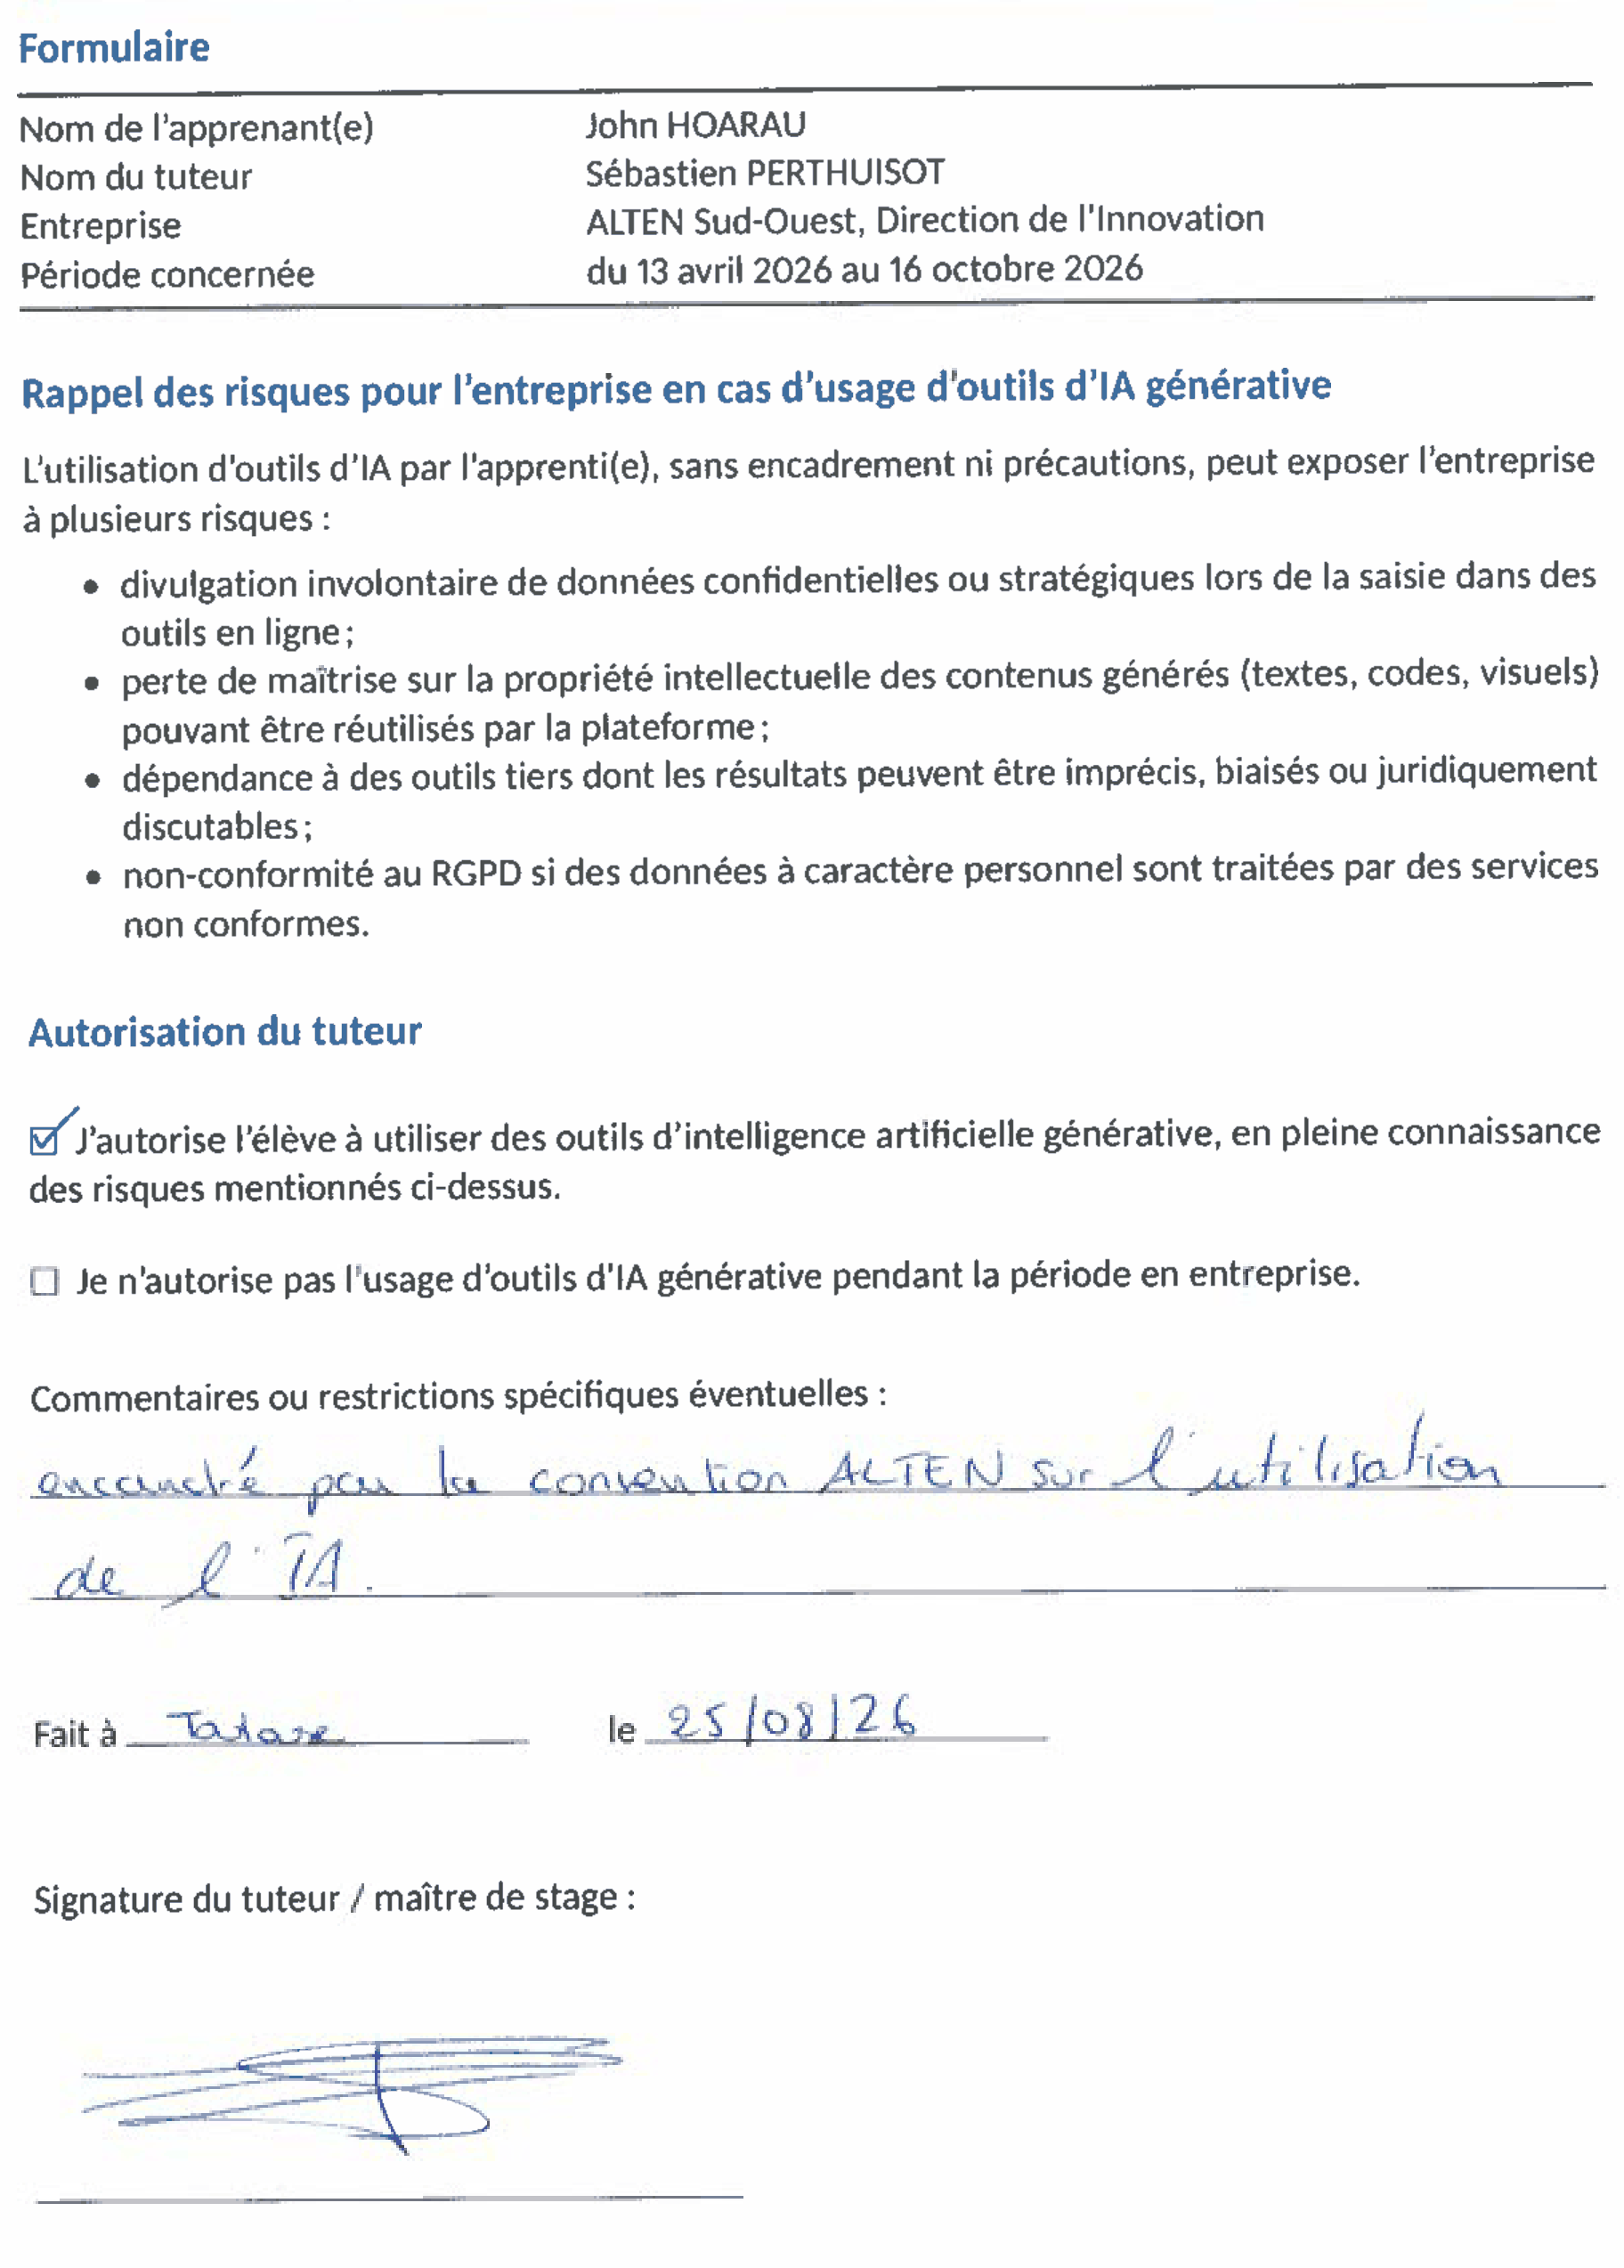
\includegraphics[width=0.88\linewidth]{Images/autorisation_ia_signee.png}
    \caption[Signed authorisation of AI use]{The authorisation form, signed.}
    \label{fig:autorisation_ia}
\end{figure}

\subsection*{Declared use of AI tools in this mission}

For transparency, and independently of the authorisation above, the use made of generative AI
during this internship is declared here in full.

Large language models were used in two distinct capacities, which should not be confused.

First, as an \emph{object of study}. The eight declarants of the experimental campaign
reported in Section~\ref{sec:realisation_experience} are language-model agents. This is an
experimental design choice, stated as such throughout the report, and its consequences for
the validity of the results are discussed rather than glossed over.

Second, as a \emph{writing aid}, for language correction and document formatting. Every
scientific claim, every numerical result and every interpretation in this report is my own,
and I am able to justify and explain each of them. Every figure was produced either by the
project's own code or by hand. No confidential ALTEN data was submitted to any external
service in the course of that assistance.

\section{Detailed Planning}
\label{app:planning}

This appendix expands the schedule of Section~\ref{sec:planning} into the weekly rhythm that
produced it, and records the two planning revisions made during the mission.

\subsection*{Weekly cadence}

Table~\ref{tab:cadence} lists the standing meetings that structured every week of the
mission.

\begin{table}[htbp]
\centering
\caption{Standing weekly meetings}
\label{tab:cadence}
\small
\begin{tabularx}{\linewidth}{>{\raggedright\arraybackslash}p{2.2cm} >{\raggedright\arraybackslash}p{3.4cm} >{\raggedright\arraybackslash}p{3.2cm} X}
\toprule
\textbf{Day} & \textbf{Meeting} & \textbf{With} & \textbf{Purpose} \\
\midrule
Monday & Planning, Green Supply Chain activity & \'E.\ Lardy & Set the objective for the
week \\
Tuesday & Scrum & \'E.\ Lardy & Progress, blockages \\
Wednesday & Scrum & \'E.\ Lardy & Progress, blockages \\
Wednesday & Supply chain regular point & S.\ Perthuisot & Scientific direction and
arbitration \\
Thursday & Scrum & \'E.\ Lardy & Progress, blockages \\
Friday & Demonstration & \'E.\ Lardy, S.\ Perthuisot & Show working output, not describe it
\\
\bottomrule
\end{tabularx}
\end{table}

Six standing contact points a week is a demanding cadence for a research placement. Its
effect was to bound how long any misconception could survive: the Friday demonstration in
particular required something to be shown rather than reported, which repeatedly exposed
gaps between what was believed to work and what did.

\subsection*{Planning revisions}

\paragraph{June: validation over extension.}
The original plan allocated the second half of the mission to widening the model's scope. It
was reallocated to validating what already existed. The argument accepted at the regular
point was that extending an unvalidated model compounds risk rather than reducing it. This
revision is why the mission produced a measured result rather than a larger unmeasured
system.

\paragraph{July: substitution of the campaign population.}
The campaign was designed for eight human consultants across nine working days. When that
could not be secured within the mission window, the protocol was executed with isolated
agents instead. The record format was deliberately identical, so the substitution changed the
population without changing the instrument. Every behavioural conclusion was weakened
accordingly in the reporting rather than being stated at the strength the original design
would have supported.

\subsection*{Comparison of planned against actual}

Table~\ref{tab:planning_ecart} compares the time allowed for each phase with the time it
actually took.

\begin{table}[htbp]
\centering
\caption{Planned against actual, by phase}
\label{tab:planning_ecart}
\small
\begin{tabularx}{\linewidth}{>{\raggedright\arraybackslash}p{3.6cm} >{\centering\arraybackslash}p{2.2cm} >{\centering\arraybackslash}p{2.2cm} X}
\toprule
\textbf{Phase} & \textbf{Planned} & \textbf{Actual} & \textbf{Comment} \\
\midrule
Framing & 3 weeks & 2.5 weeks & On plan \\
First urgency model and pipeline & 6 weeks & 5.5 weeks & Stopped early once judged
inadequate \\
Capacity from imagery & 4 weeks & 8 weeks & Ran in parallel; the original objective proved
unreachable and the problem had to be reframed \\
SupplyScore build & 4 weeks & 2 weeks & Interfaces already established by the abandoned
pipeline \\
Experimental design & 2 weeks & 3 weeks & Freezing the protocol properly took longer than
allowed \\
First campaign and diagnosis & 3 weeks & 3 weeks & On plan \\
Independent validation & \emph{unplanned} & 3.5 weeks & Added after the diagnosis:
repair, second
chain, baseline comparison \\
Calibration campaigns & 4 weeks & \emph{planned} & 25 August to 19 September \\
Vision model & 3 weeks & \emph{planned} & 7 to 26 September, overlapping the above \\
Scientific report and defence & 3 weeks & \emph{planned} & 28 September to 16 October \\
\bottomrule
\end{tabularx}
\end{table}

The overall schedule held. Two overruns had to be absorbed. The imagery workstream took twice
its allowance because the original objective turned out to be physically unreachable and the
problem had to be reframed before anything could be built; the time came out of the
SupplyScore build, which the abandoned pipeline had already de-risked. The validation phase
was unplanned entirely and consumed three and a half weeks, released by the framing and build
phases finishing early. The one systematic underestimate was the effort required to freeze an
experimental protocol to a standard where the hypotheses could not later be adjusted, which
took half again the time allowed and was worth every day.

\subsection*{What the remaining two months carry}

The mission runs to 16 October and this report is submitted on 24 August. The remaining time
carries no new construction, and it is loaded to roughly the same weekly effort as the phases
already closed.

\begin{enumerate}
    \item \emph{Calibration campaigns, 25 August to 19 September.} New serious-game chains,
    built the way the airframer chain was, run to widen the evidence base. This is the single
    action that moves every sample-bound figure in Section~\ref{sec:conclusion_limites}, and
    it is also what allows the forecast layer to be recalibrated on more than one scenario.
    \item \emph{Vision model, 7 to 26 September, overlapping the above.} The facade
    segmentation model of Section~\ref{sec:realisation_volume} carries a global bias of
    $-35\%$ on the derived dock count. Annotated volume, not architecture, drove every gain
    measured so far, so the work is data collection and re-training rather than redesign.
    \item \emph{Scientific report and defence, 28 September to 16 October.} The
    \emph{Bilan Scientifique et Technique} that capitalises the whole internship for the
    programme, and the defence.
\end{enumerate}

Any rate quoted in this report may therefore move. The constructions and the diagnoses will
not.

\section{Detailed Competency Evidence}
\label{app:competences}

This appendix gives the evidence behind Table~\ref{tab:competences}, competency by
competency, so that each claim can be checked against something in the record rather than
taken on assertion.

\paragraph{CI1 -- Analysis, synthesis, curiosity, creativity and innovation, approaching a
problem systemically and across disciplines.}
The measurement built during this mission required combining four fields that do not normally
cite one another: deadline-driven value from operations research, the mere-urgency effect
from behavioural science, probabilistic aggregation, and the software architecture needed to
make the result auditable. The contribution claimed is not any one of them but the
combination, which Section~\ref{sec:gap} shows to be absent from the reviewed literature.

\paragraph{CI3 -- Working in an international and intercultural context.}
The mission was conducted, documented and defended in English, within a double-degree
programme with a British university. A colleague on the same research programme worked in
English on the adjacent representation problem, and the weekly demonstration was the point at
which the two strands had to be made intelligible to each other.

\paragraph{CI5 -- Identifying and solving complex or research problems, mobilising scientific
and technical knowledge and external resources.}
The subject was a research problem with no established answer. The word \emph{external} also
applies literally: as recorded in Section~\ref{sec:risques}, the company holds no journal
subscriptions, so every source in the state of the art was retrieved through university
credentials.

\paragraph{CE3 -- Leading, steering and controlling a project to reach its objectives, in
cost, deadline, performance and risk.}
Six phases with dated milestones; a weekly cadence of six standing meetings; a documented
mid-mission replanning that traded scope for validation; and a risk register of four items of
which three materialised and were handled. Cost is the one dimension not exercised, since no
budget was managed.

\paragraph{CE4 -- Taking the socio-ecological transition into account.}
Carbon is one of the six blocks of the model, ranked alongside cost and delay rather than
applied as a correction, and the programme itself falls within the share of ALTEN's R\&D
devoted to environmental innovation (Section~\ref{sec:rse}). The honest qualification, stated
in Section~\ref{sec:conclusion_limites}, is that this block turned out to be the least
exercised of the six for want of data.

\paragraph{CE5 -- Researching, selecting, qualifying and diffusing information, adapting it
to its context.}
The qualifying step is the one worth evidencing: a candidate dataset was inspected before use
and rejected on three measurable signatures of synthetic data, and the node it would have fed
was driven by calibrated events instead. On diffusion, the same work was written three ways
for three audiences: a scientific report for the company, a research thesis for the partner
university, and this mission report.

\paragraph{CST1 -- Defining an engineering strategy by choosing methods and tools suited to a
known or poorly known context.}
The assignment as signed covered five workstreams. Converging it onto one defensible
contribution, and recording the boundaries explicitly rather than leaving them implicit, was
the first engineering decision of the mission. The second was abandoning the initial urgency
formulation once it proved unable to represent a node on schedule but out of capacity.

\paragraph{CST2 -- Modelling and simulating a system, and capitalising the information and
knowledge produced.}
The six-block model with its bidirectional propagation, the campaign that simulates a
documented historical crisis over nineteen turns, and a derivation pipeline that regenerates
every reported figure from raw artefacts so that no number in any of the three deliverables
is transcribed by hand.

\paragraph{CST7 -- Designing and building models, methods and tools to aid engineering and
improve business processes, including in a research and development perspective.}
The delivered application and the experimental protocol were both built to be continued
rather than to end with the placement: a documented architecture, an automated test suite, a
frozen and hashed protocol, and a written record of what the next steps are and in what
order.


\end{document}
